\chapter{Evolution of Environmental Sensing through DNA Supercoiling}
\chaptermark{Evolution of Environmental Sensing through DNA SC}
\label{chap:alife}

This chapter presents the proof-of-concept version of the \emph{EvoTSC} model, and the first results that I obtained with that version of the model: I show that the evolution of differentiated expression levels in different environments is possible when gene expression is only regulated by the transcription-supercoiling coupling.
The text of the chapter is an edited version of an article published in the \emph{Artificial Life} journal~\citep{grohens2022a}.

\paragraph{}
Both the importance of gene regulation via supercoiling and the detailed mechanisms of the transcription"=supercoiling coupling, at the local scale, have already been studied extensively in the literature (see Section~\ref{sec:background:sc}).
However, a thorough analysis of the effect of the transcription-supercoiling coupling on gene expression at the whole-genome scale -- and of its possible evolutionary use by natural selection -- remains lacking, in particular in the dense prokaryotic genomes, in which large groups of genes are likely to interact through this coupling.
In this work, we describe a new model which incorporates a high-level model of global supercoiling regulation and of the transcription"=supercoiling coupling within an \emph{in silico} experimental evolution setting.
Using this model, we first investigate the non-linear variation in gene transcription levels at the whole-genome scale in response to variations in the global supercoiling level.
Then, we study the evolutionary trajectory of gene activation patterns in individuals subjected to different environments.

We show that in our model, a genome-scale gene interaction network emerges from local supercoiling-mediated interactions, and creates a reaction norm in response to the change of a single parameter, the global supercoiling level, caused by different environments.
Moreover, we demonstrate that, using genomic inversions as the only mutation operator, and therefore only changing the relative positions and orientations of genes on the genome, evolution can select genomes displaying qualitatively different phenotypes in different environments characterized by different global supercoiling conditions.

%This article is an extended version of~\cite{grohens2021}.

\section{A Genome-Wide Model of the Transcription-Supercoiling Coupling}
\label{sec:alife:indiv_model}

\begin{figure}[H]
\centering
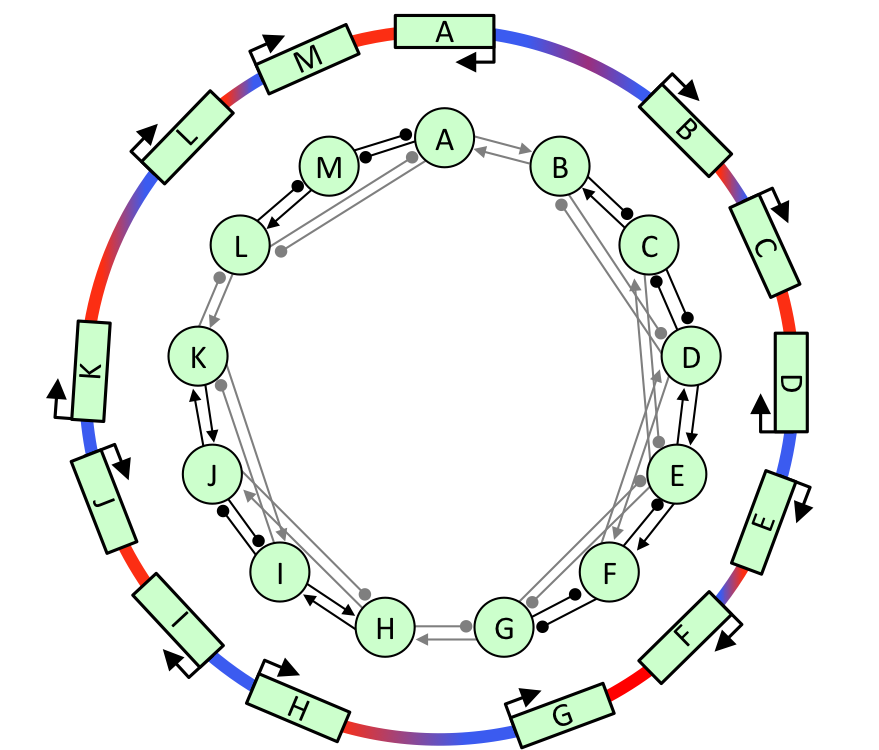
\includegraphics[width=0.75\textwidth]{alife/img/reseau.png}
\caption[Hand-drawn genome and local interactions resulting from the TSC]{Genes along an example genome and local variations in supercoiling (outer ring), and the associated gene interaction network (inner ring).
The outer ring color shows locally high ($\sigma > \sigma_0$, red) or low ($\sigma < \sigma_0$, blue) supercoiling levels due to gene transcription.
In the inner ring, closer genes interact more strongly (black arrows) than genes that are farther apart (gray arrows), either positively or negatively depending on their relative orientations.}
\label{fig:alife:network}
\end{figure}

%In this paper, we present a model which aims at studying the genome-wide effect of the transcription-supercoiling coupling in bacteria, expanding upon previous work which only considered local interactions.
%In gene-dense genomes such as prokaryotic ones, transcription-supercoiling coupling between nearby genes is likely to give rise to a genome-wide transcriptional network, the topology of which depends on relative gene distances and orientations.

Our model consists in an individual-based simulation, written in Python.
Its source code is available at \url{https://gitlab.inria.fr/tgrohens/evotsc/-/tree/alife-journal}.
It is also preserved for \href{https://archive.softwareheritage.org/swh:1:rev:6fc36abc1661c295782886647c37ef05ffb9d357}{long-term archival} using the Software Heritage online archive~\citep{dicosmo2020}.
An individual in the model is represented by a circular genome (representative of most bacterial genomes), comprising a fixed number of genes, separated by non-coding intergenic regions.
Each gene is described by the following characteristics: its locus on the genome, its orientation, and its basal transcription (or expression) level.
As we are mainly interested in the interplay between supercoiling and transcription, we voluntarily do not make the difference between gene expression levels, understood as mRNA or protein concentrations, and transcription levels, the immediate rate of mRNA
production.
Indeed, assuming a separation of timescales between the fast equilibrium of the transcription-supercoiling coupling, and the slow degradation of mRNAs, the concentration of a given mRNA is directly proportional to the transcription rate of its source gene.

Figure~\ref{fig:alife:network} illustrates the role played by the transcription-supercoiling coupling in an example genome.
It includes the local supercoiling variations due to gene transcription, and the resulting gene interaction network, with each gene possibly activating or inhibiting its neighbors, depending on their relative orientations.
Importantly to our approach, here genes do not interact only with their closest neighbors, but also with more distant genes, as is likely to be the case in the gene-rich bacterial genomes: \emph{E. coli} gene promoters are around one thousand base pairs apart~\citep{peter2004}, and the transcription-generated supercoiling propagates around a few thousand base pairs on each side of the transcription site~\citep{postow2004}.


\subsection{Mathematical Description of the Model}

We model the transcription-supercoiling coupling between an individual's genes as a system of equations, which relate the supercoiling level at the locus of each gene $\sigma_i$ (for $i$ ranging from $1$ to $n$, the number of genes of the individual), and the expression level of every gene $e_i$.
The parameters of the system are described by the genome of the individual, as will be detailed below.

In our model, the supercoiling at a given locus on the genome depends on three factors: the individual's basal supercoiling level $\sigma_{basal}$, the variation in supercoiling due to environmental conditions $\sigma_{env}$, and the variation in supercoiling due to the transcription of the neighboring genes.
We compute this local variation in supercoiling at the locus of each gene with the help of a gene interaction matrix, whose coefficient at position $(i, j)$ describes the influence of gene $j$ on gene $i$.
The coefficients are given by the following equation:

\begin{equation}
\frac{\partial\sigma_{i}}{\partial e_j} = \eta\cdot c \cdot\max(1-\frac{d(i, j)}{d_{max}}, 0)
\label{eq:dsde}
\end{equation}
%This interaction level abstracts the influence of local supercoiling into a single value, which reflects the positive or negative influence of each gene on the transcription level of the other genes in the genome.

More precisely, the interaction level between two genes depends on the relative orientation of the genes, as the transcription of a gene increases supercoiling at the locus of downstream genes and decreases supercoiling at the locus of upstream genes (remember that an increase in supercoiling means a decrease in transcription).
Therefore, we choose $\eta = 1$ if gene $i$ is downstream of gene $j$ and $\eta = -1$ otherwise (if $i=j$, $\eta = 0$ as a gene does not interact with itself).
The interaction level also depends on gene distance, as genes that are further apart on the genome interact less strongly, so the strength of the interaction linearly decreases with the intergenic distance $d(i, j)$, and reaches 0 when $d(i, j) = d_{max}$, the maximum distance above which the interaction vanishes.
Finally, an interaction coefficient $c$ is applied to adjust the strength of the coupling.

Using this interaction matrix, we compute the level of supercoiling $\sigma_i$ at the locus of every gene, which depends on the transcription level of all the other genes, on the basal supercoiling level, and on the environmental supercoiling level:

\begin{equation}
\sigma_i = \sigma_{basal} + \sigma_{env} + \sum_{j=1}^n\frac{\partial\sigma_{i}}{\partial e_j}e_j
\label{eq:alife_sigma}
\end{equation}

The transcription level $e_i$ of every gene as a function of total supercoiling is then modeled with a sigmoidal activation curve, following~\cite{elhoudaigui2019}.
The equation is given below:

\begin{equation}
e_i = \frac{1}{1 + e^{(\sigma_i - \sigma_0)/\epsilon}}
\label{eq:transcr}
\end{equation}

In this equation, $\sigma_0$ is a parameter that represents the inflexion point of the sigmoid, that is the supercoiling level at which the gene is at half its maximum transcription rate, and $\epsilon$ a scaling factor that represents the strength of the dependence of the transcription level on the supercoiling level.

Finally, in order to obtain the phenotype of an individual, we numerically compute a solution to the system of equations~\ref{eq:alife_sigma} and~\ref{eq:transcr}, using a fixed point algorithm.
This solution represents the state (of gene expression and supercoiling at every locus) towards which the individual would converge over time.
Let $f(e_i)$ be the function that computes new supercoiling levels $\sigma'_i$ from $e_i$ using equation~\ref{eq:alife_sigma}, and then computes new expression levels $e'_i$ from the new $\sigma'_i$ using equation~\ref{eq:transcr}, and finally returns $e'_i$.
In order to compute a fixed point of $f$, that is a set of transcription levels $e_i^*$ such that $f(e_i^*) = e_i^*$, we start with basal transcription levels $e_i^0$ (that are a property of each gene), and iterate the sequence $e_i^{t+1} = \frac{1}{2}(e_i^t + f(e_i^t))$, until the difference between two successive iterations is below a given threshold.
In our setting, this algorithm has empirically always converged to a solution that is a stable fixed point of the function, and that is therefore interpretable from a biological perspective.

\begin{figure}[H]
\centering
\begin{subfigure}[t]{0.42\textwidth}
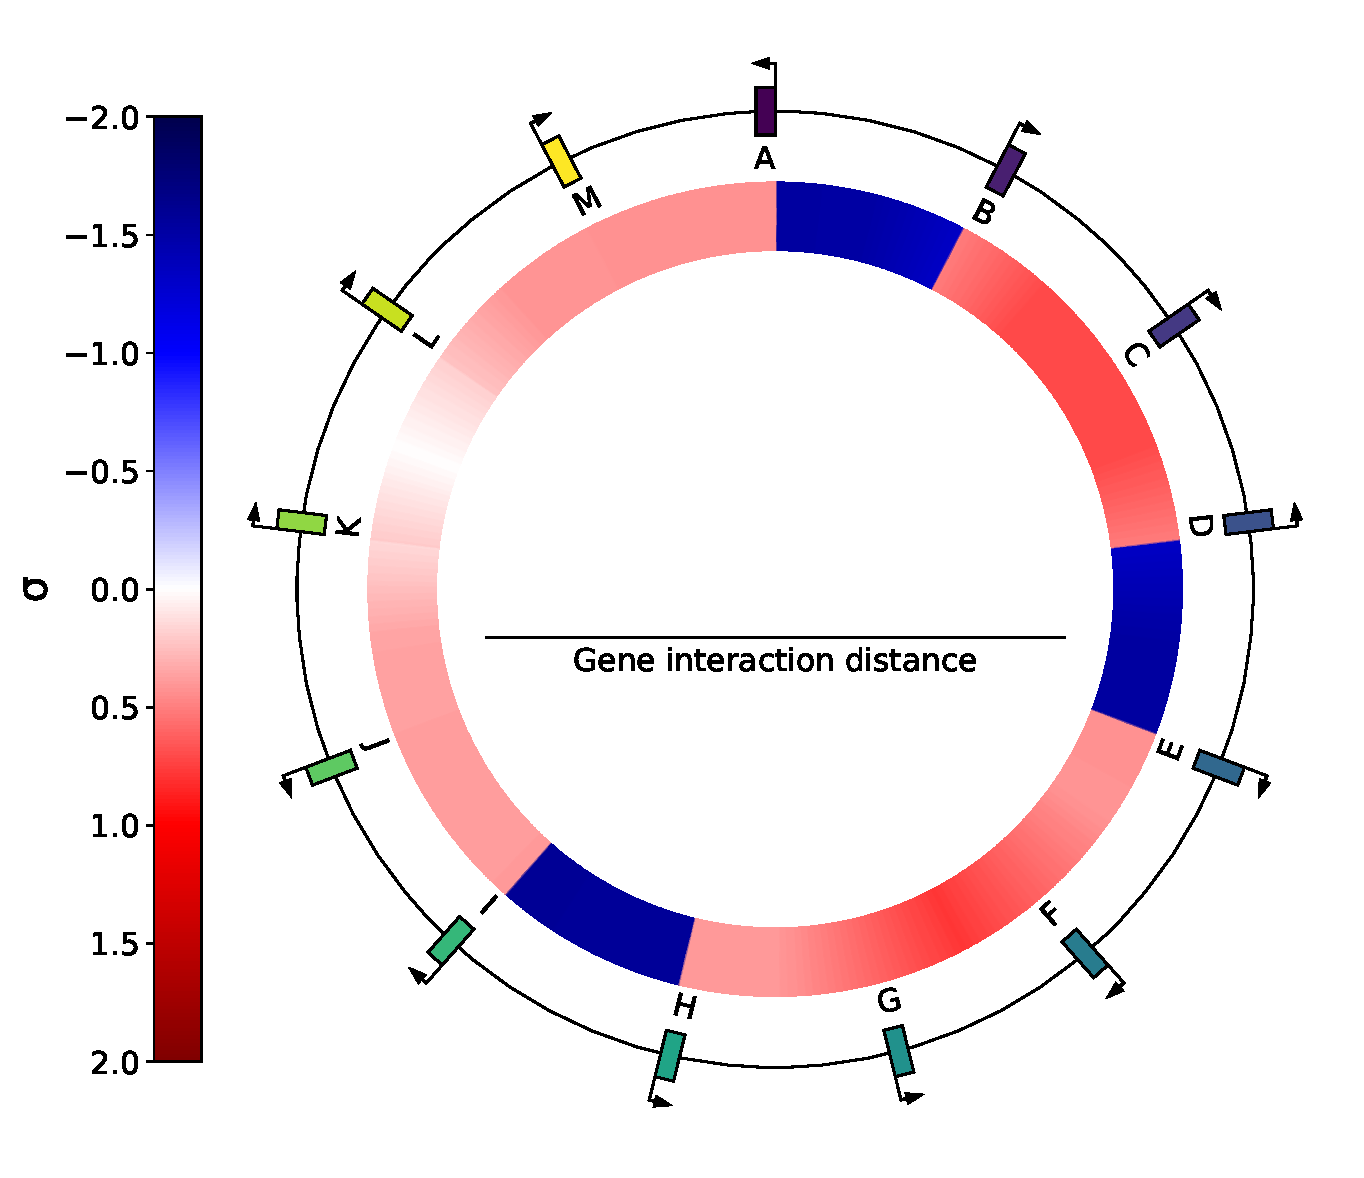
\includegraphics[width=\textwidth]{alife/img/13genes_genome.pdf}
\label{subfig:alife:13genes_genome}
\end{subfigure}
\begin{subfigure}[t]{0.56\textwidth}
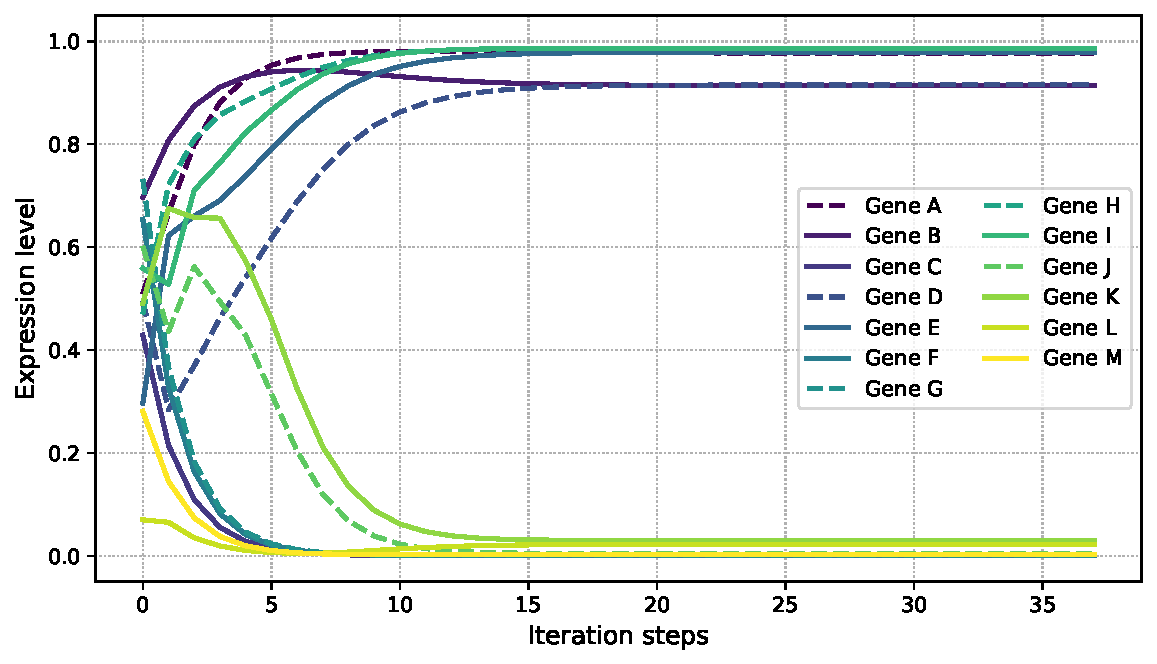
\includegraphics[width=\textwidth]{alife/img/13genes_expr_level.pdf}
\label{subfig:alife:13genes_expr}
\end{subfigure}
\caption[Example individual in the proof-of-concept model]{Left: genome (outer ring) and stable state level of supercoiling $\sigma$ (inner ring) of an example individual with 13 genes in the model.
Right: transcription levels of the individual's genes during the iterations of the fixed point computation, in an environment given by $\sigma_{env} = 0.05$.
Solid lines represent genes in forward orientation, and dashed lines represent genes in reverse orientation.}
\label{fig:alife:13genes}
\end{figure}

Figure~\ref{fig:alife:13genes} shows the genome (left, outer ring) of an example individual with a genome of 13,000 bp and $n=13$ genes evenly spaced along the genome, and with a basal supercoiling of $\sigma_{basal} = -0.06$.
The basal transcription level of each gene is randomly chosen between 0 and 1, and all the iterations of the fixed point algorithm that result in the final gene transcription levels are shown on the right.
In this individual, the non-linear effect of the interaction between neighboring genes is clearly visible.
Indeed, six genes (A, B, D, E, H, and I) end up at a high transcription rate at the fixed point (or solution) of the system, while the others end up at low transcription rates.
These activated genes can be grouped into 3 pairs (A and B, D and E, H and I), all of which are pairs of adjacent genes in divergent orientations.
Even though gene D has a low (around 0.3) basal transcription rate, it eventually reaches a high transcription state because of its positive interaction with gene E.
Conversely, genes F and G start with a high transcription rate, but are repressed by their neighbors H and E, and are therefore silenced as the system converges.
We can also observe complex behaviors in the model, as the gene expression levels pass through very different states during convergence to the solution.
Indeed, the transcription level of gene K initially increases due to its interaction with gene J, but both genes end up in a low transcription state, as they are inhibited by the very active gene I.
The final supercoiling level along the genome (left, inner ring) moreover demonstrates the effect of the transcription-supercoiling coupling on local supercoiling.
Highly transcribed genes, such as A and B, generate a large variation in the supercoiling level on their upstream and downstream sides, and the positive feedback loop between genes in divergent pairs is made clear by the very high negative value of the supercoiling level between each of the genes in these two pairs.


\subsection{Effect of the Environmental Supercoiling on Gene Activation Levels}
\label{sec:alife:env_model}

\begin{figure}[H]
\centering
\begin{subfigure}[t]{0.28\textwidth}
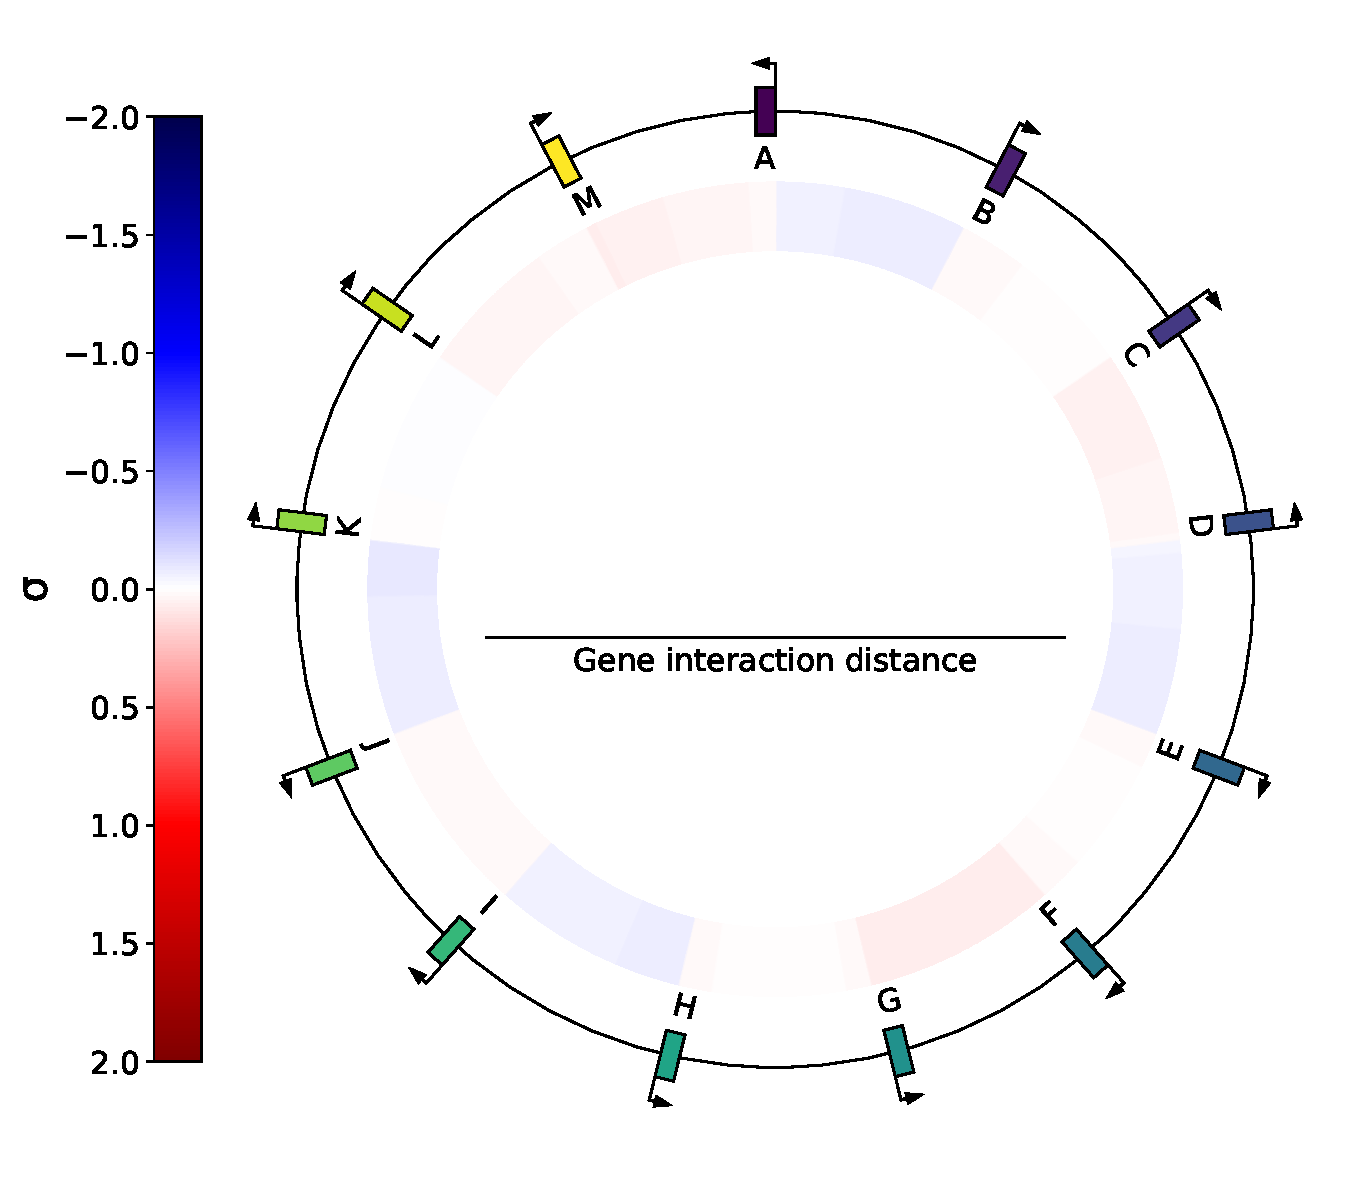
\includegraphics[width=\textwidth]{alife/img/13genes_genome_3.pdf}
\label{subfig:alife:genome_3}
\end{subfigure}
\hspace{-3mm}
\begin{subfigure}[t]{0.24\textwidth}
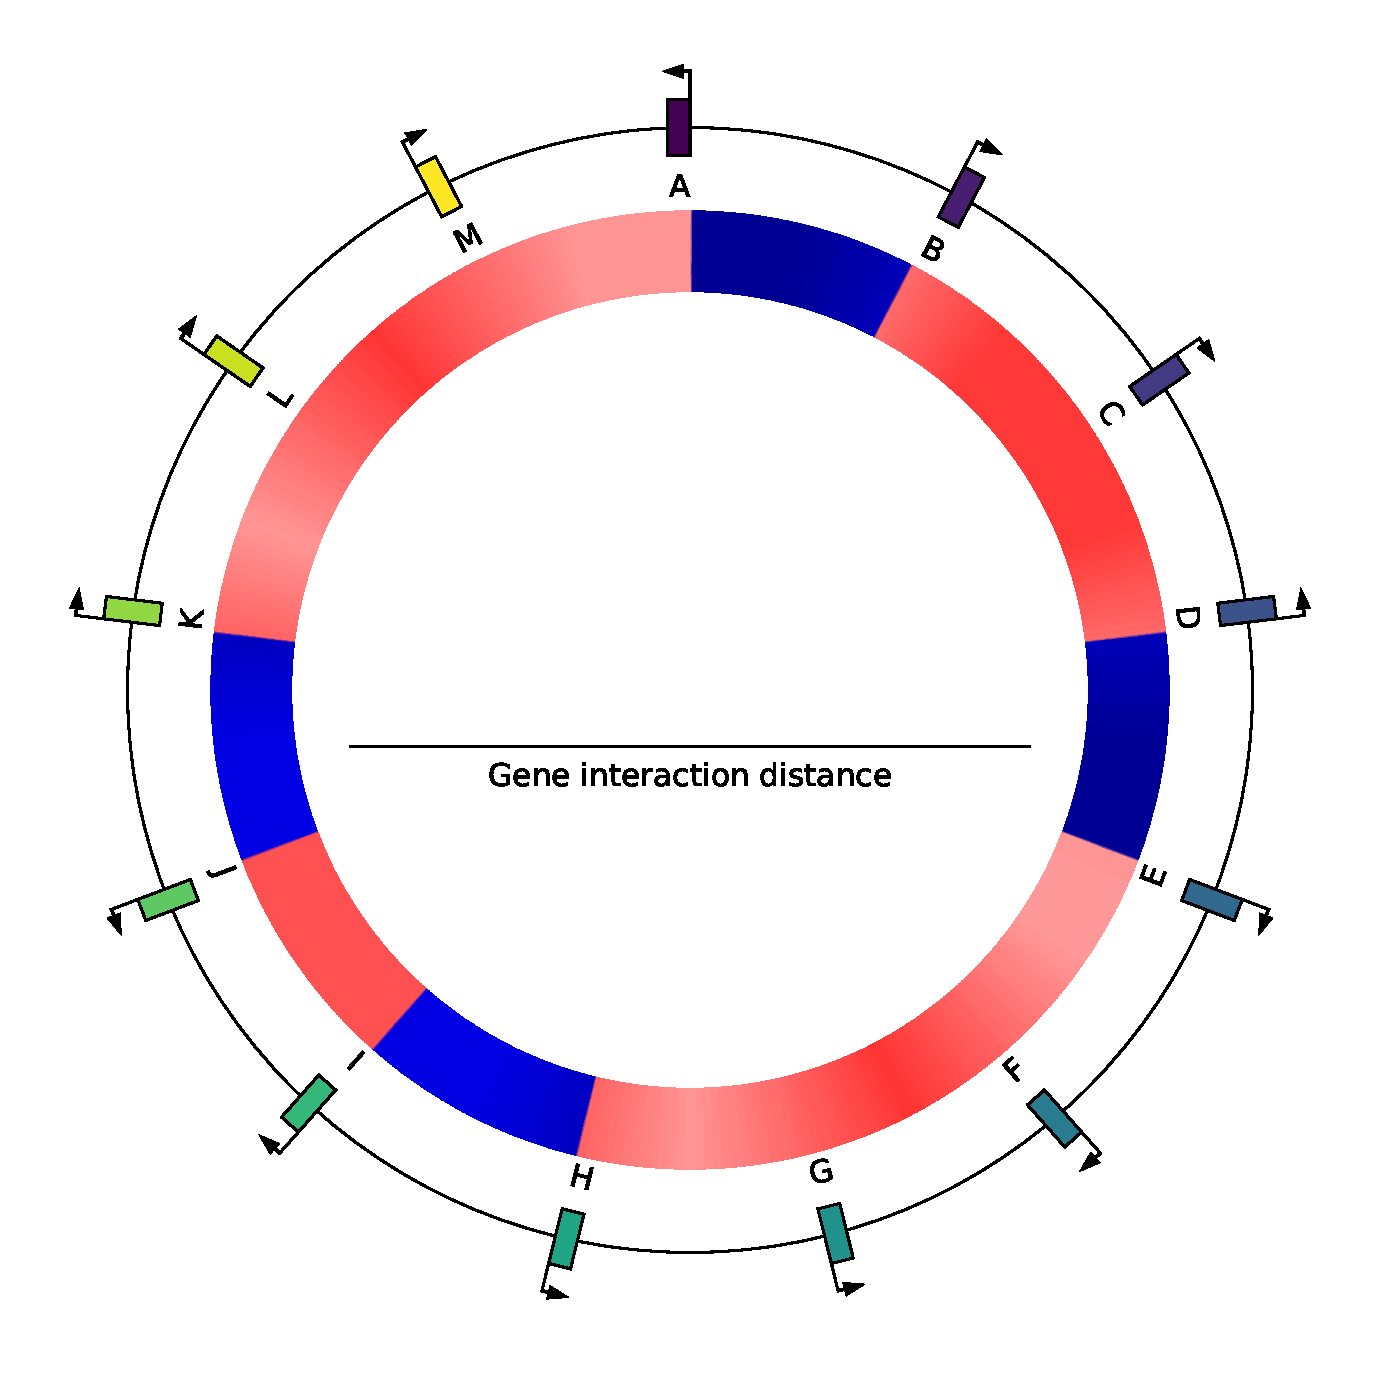
\includegraphics[width=\textwidth]{alife/img/13genes_genome_2.pdf}
\label{subfig:alife:genome_2}
\end{subfigure}
\hspace{-3mm}
\begin{subfigure}[t]{0.24\textwidth}
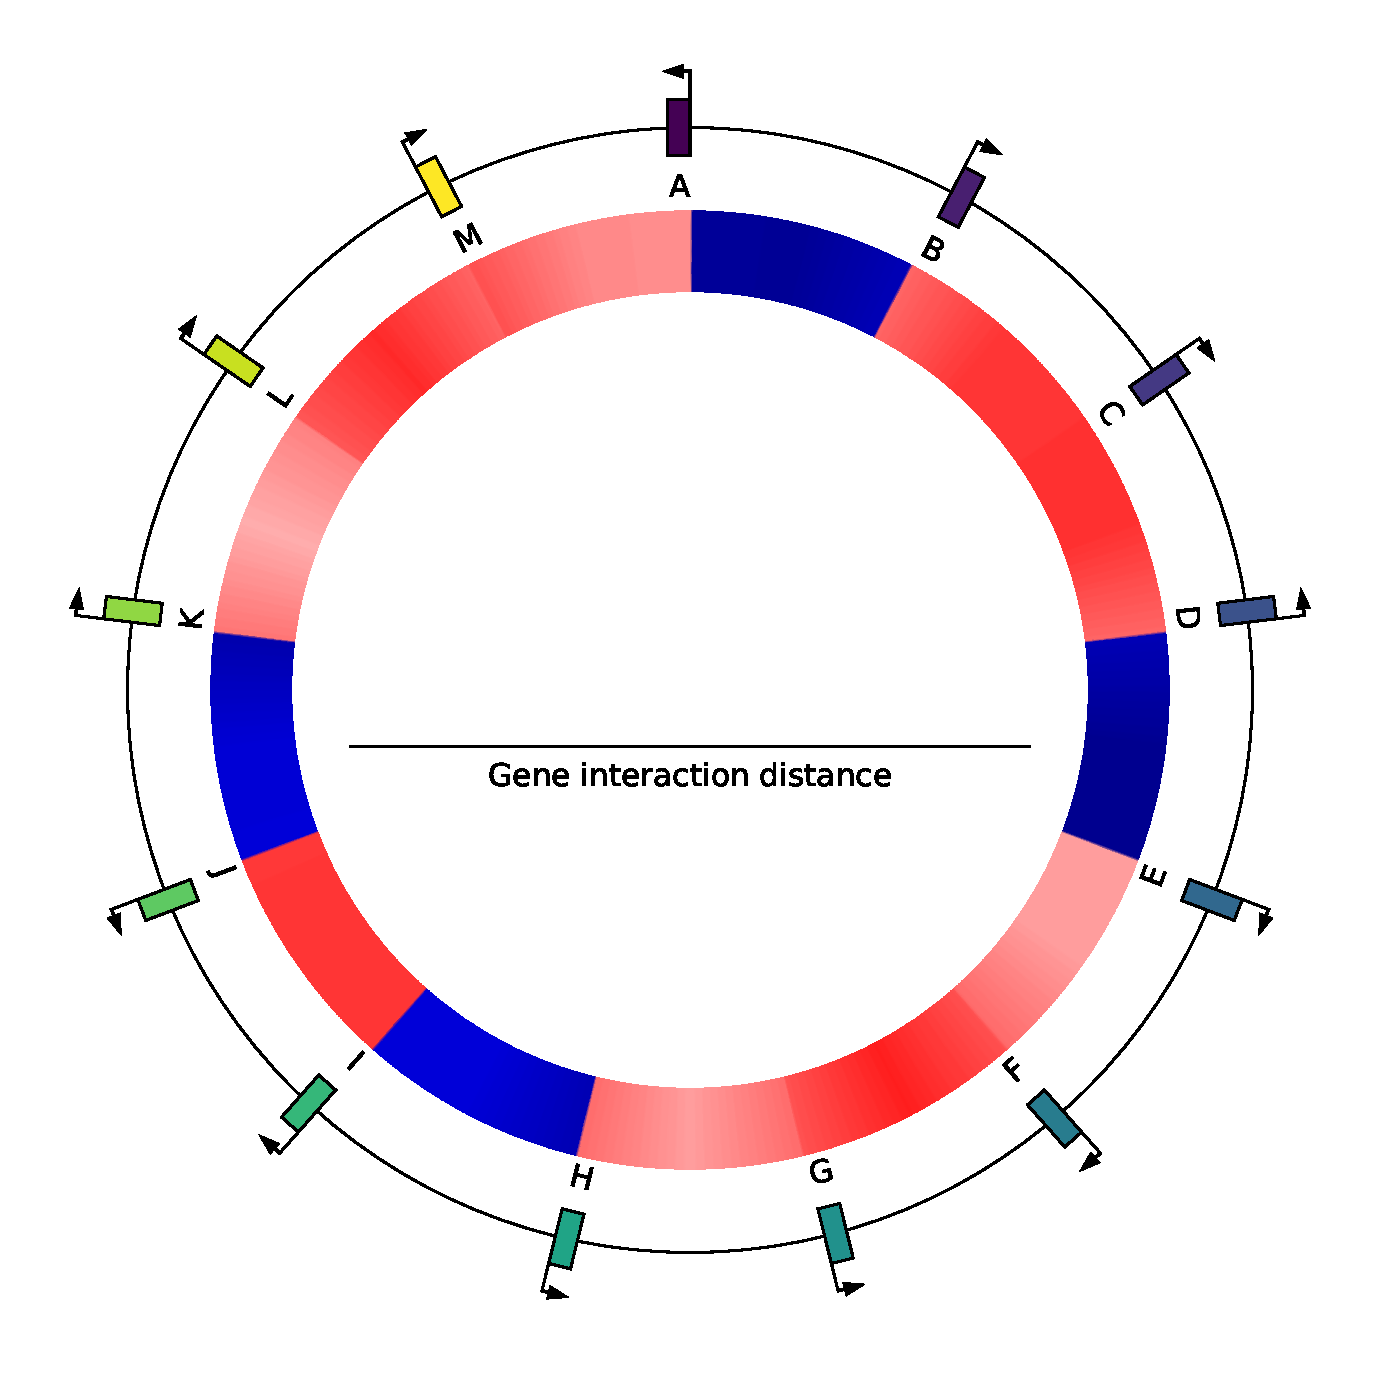
\includegraphics[width=\textwidth]{alife/img/13genes_genome_1.pdf}
\label{subfig:alife:genome_1}
\end{subfigure}
\hspace{-3mm}
\begin{subfigure}[t]{0.24\textwidth}
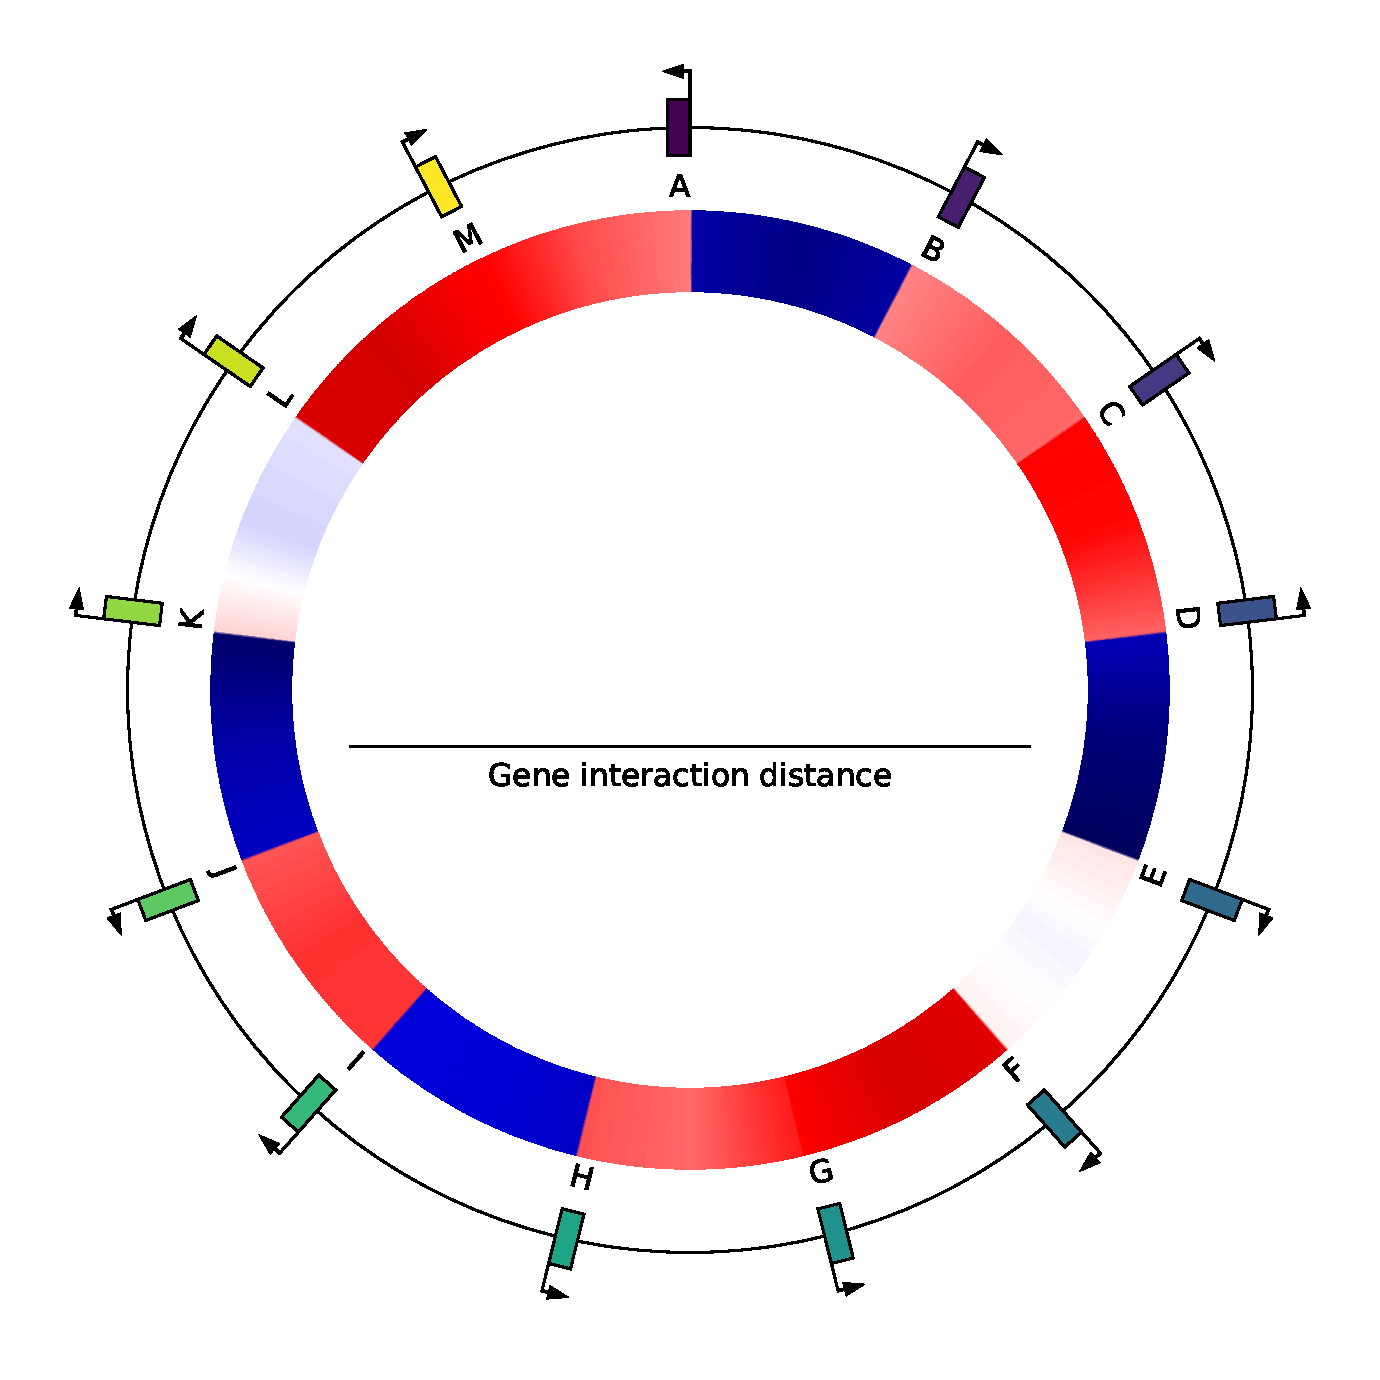
\includegraphics[width=\textwidth]{alife/img/13genes_genome_0.pdf}
\label{subfig:alife:genome_0}
\end{subfigure}
\vspace{-3mm}

\begin{subfigure}[t]{0.48\textwidth}
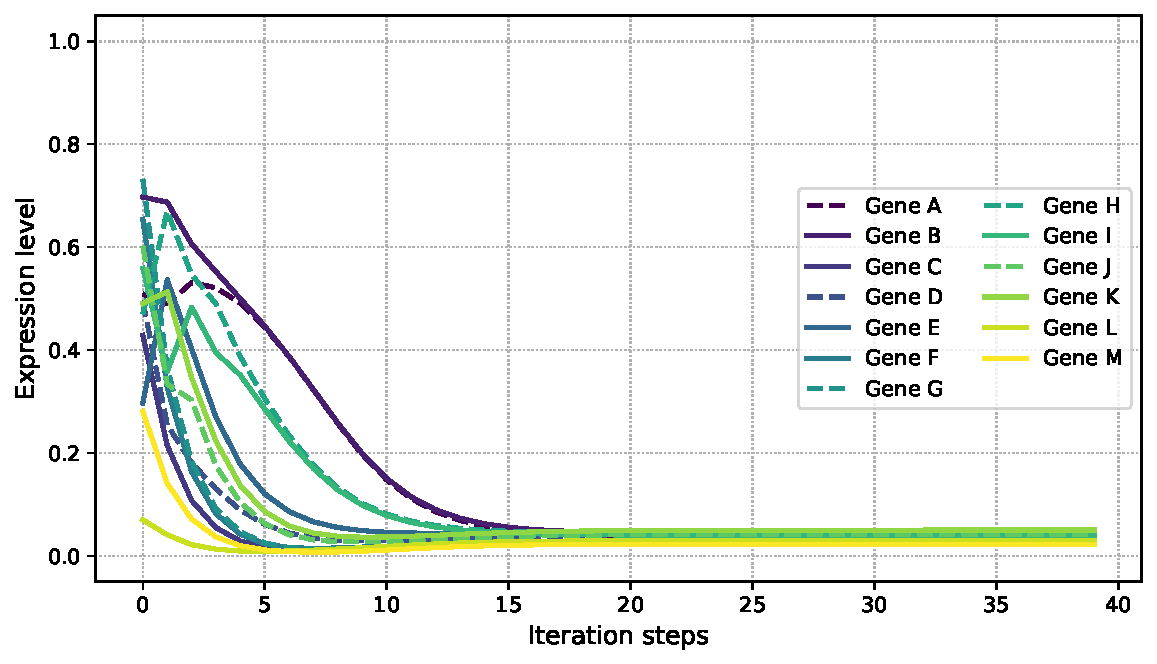
\includegraphics[width=\textwidth]{alife/img/13genes_sigma_3.pdf}
\label{subfig:alife:sigma_3}
\end{subfigure}
\begin{subfigure}[t]{0.48\textwidth}
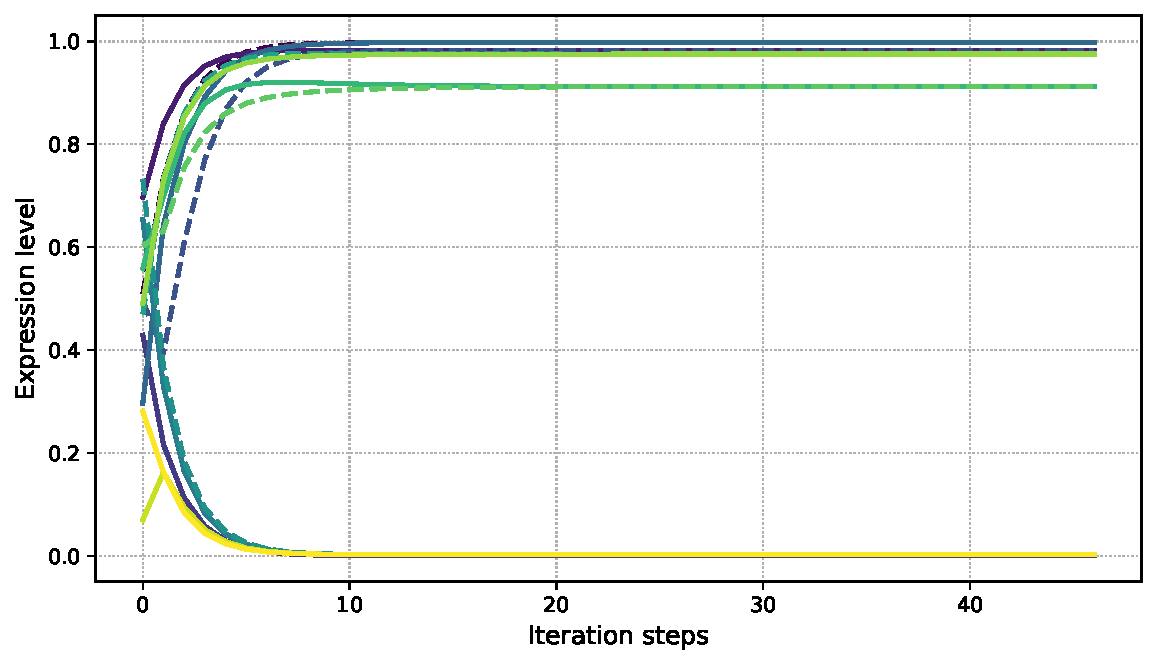
\includegraphics[width=\textwidth]{alife/img/13genes_sigma_2.pdf}
\label{subfig:alife:sigma_2}
\end{subfigure}
\vspace{-5mm}

\begin{subfigure}[t]{0.48\textwidth}
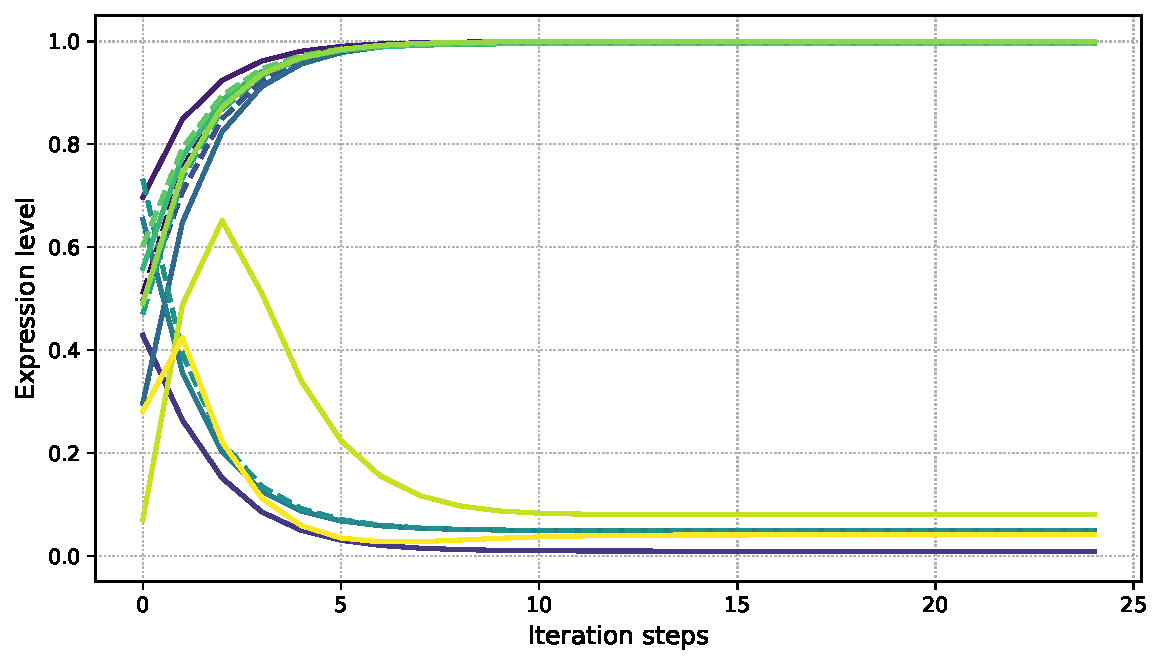
\includegraphics[width=\textwidth]{alife/img/13genes_sigma_1.pdf}
\label{subfig:alife:sigma_1}
\end{subfigure}
\begin{subfigure}[t]{0.48\textwidth}
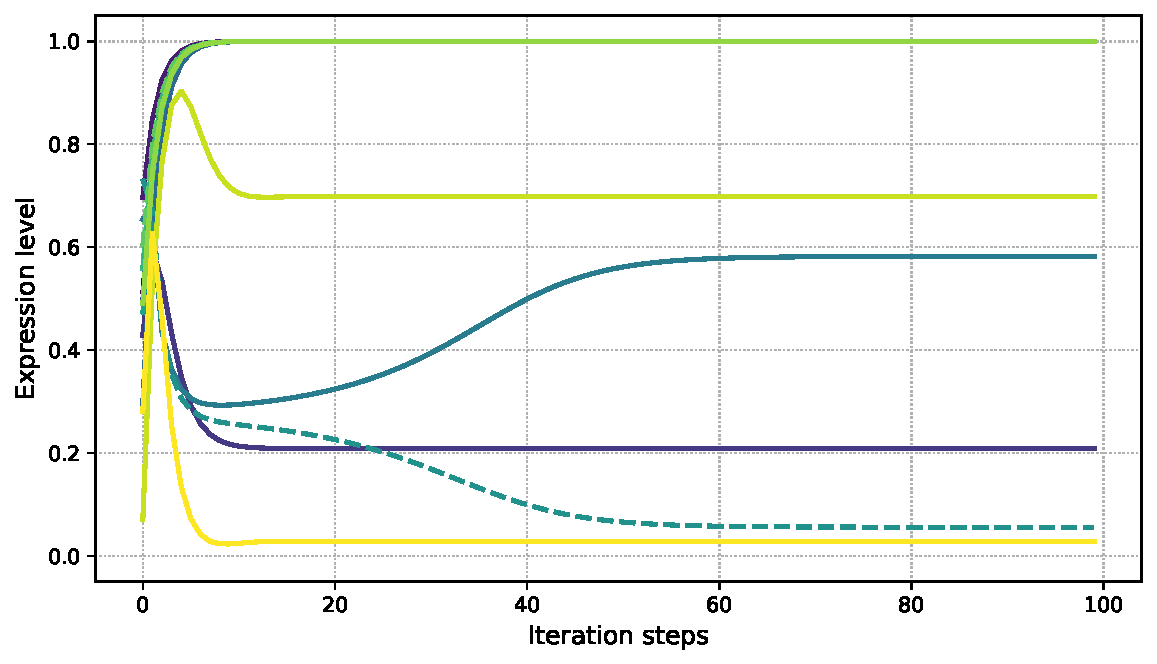
\includegraphics[width=\textwidth]{alife/img/13genes_sigma_0.pdf}
\label{subfig:alife:sigma_0}
\end{subfigure}
\caption[Influence of environmental supercoiling on the phenotype of the example individual in Figure~\ref{fig:alife:13genes}]{Influence of the environment supercoiling $\sigma_{env}$ on the stable state local supercoiling level (top row) and gene transcription levels (bottom rows) of the example individual.
From left to right and top to bottom: at $\sigma_{env} = 0.1$, no genes are activated ($e > 0.5$); at $\sigma_{env} = 0.0$ and at $\sigma_{env} = -0.1$, 8 genes are activated; at $\sigma_{env} = -0.2$, 10 genes are activated.
Lower values of $\sigma_{env}$ result in the activation of more genes, reflecting the \emph{in vivo} effect of higher negative supercoiling.}
\label{fig:alife:sigma_env}
\end{figure}

Figure~\ref{fig:alife:sigma_env} captures the influence of the environmental change in supercoiling $\sigma_{env}$ on the local supercoiling level due to the transcription-supercoiling coupling (top row) and on the repartition of genes between the activated and inhibited states (bottom rows), again using the example individual already shown in Figure~\ref{fig:alife:13genes}.
From left to right and top to bottom: at a high value of $\sigma_{env} = 0.1$, meaning that DNA is severely overwound compared to normal, no gene is activated (with an expression level $e > 0.5$) at all.
As the external influence of the environment on supercoiling decreases to $\sigma_{env} = 0$, corresponding to normal relaxation of DNA, and then to $\sigma_{env} = -0.1$, 8 out of the 13 genes of the individual reach an activated state.
Finally, for $\sigma_{env} = -0.2$, there is a strong environmental pressure towards high gene transcription levels, and most genes are indeed activated; however, even at this level of $\sigma_{env}$, some genes remain shut down, because of the high amount of positive supercoiling (in red) generated by the transcription of their neighbors.


\subsection{Influence of Relative Gene Positions on Gene Activation Levels}
\label{sec:alife:gene_pos}

\begin{figure}[H]
\centering
\begin{subfigure}[t]{0.42\textwidth}
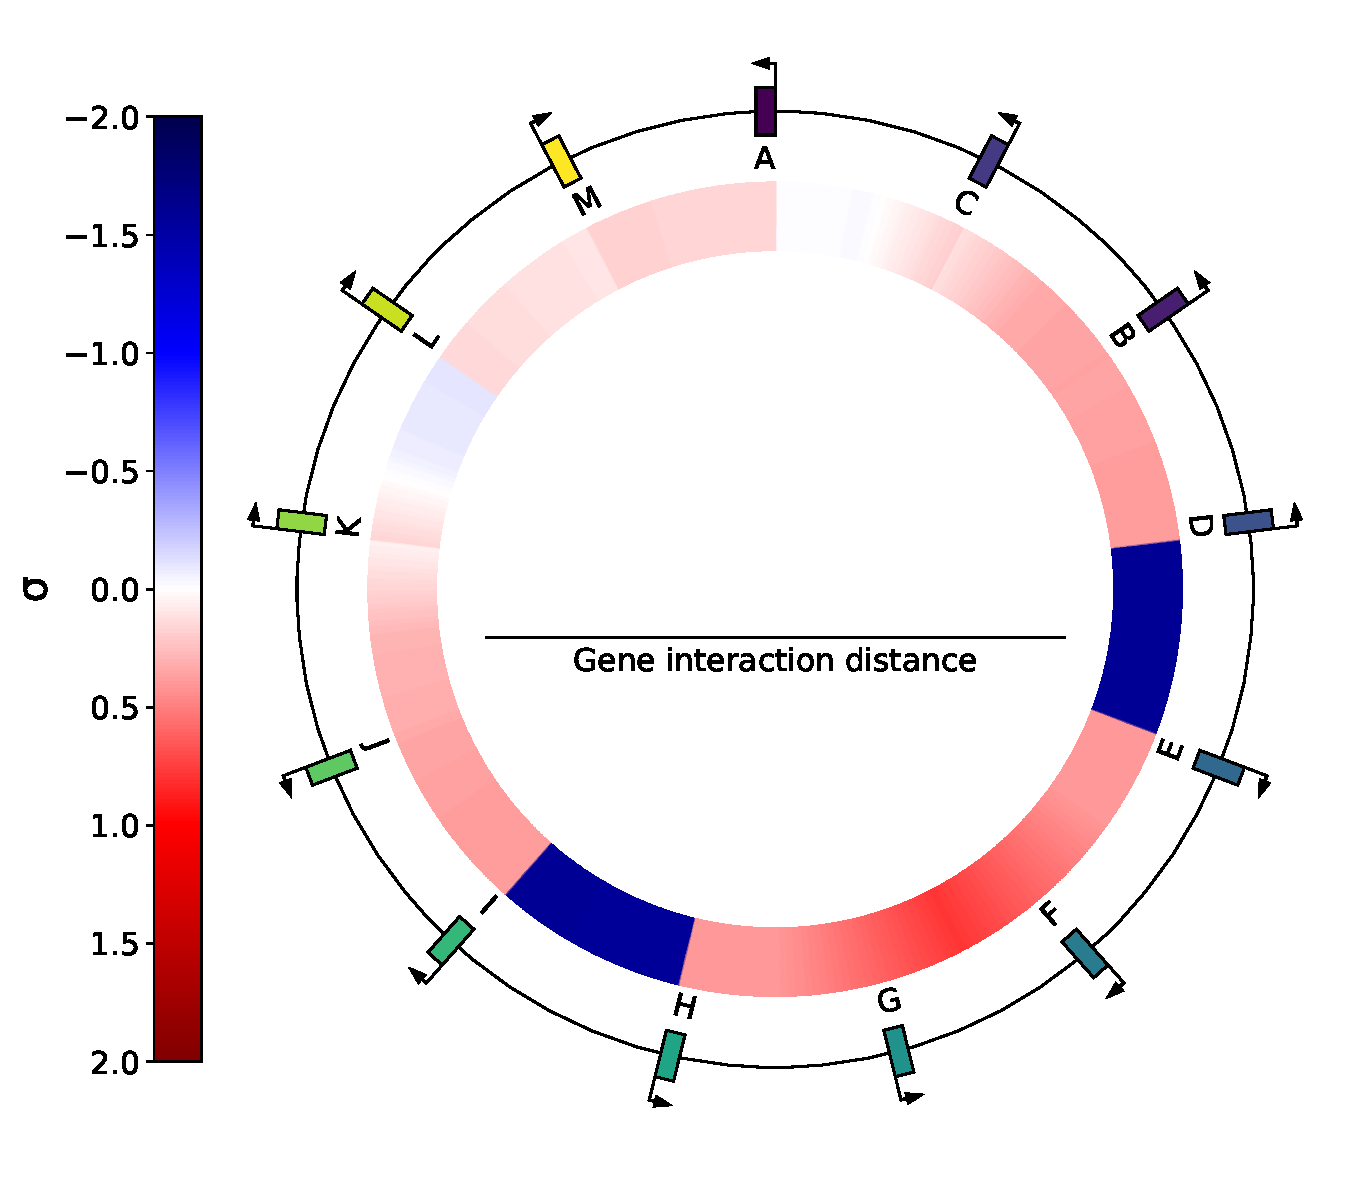
\includegraphics[width=\textwidth]{alife/img/inversion_genome.pdf}
\label{subfig:alife:inversion_genome}
\end{subfigure}
\begin{subfigure}[t]{0.56\textwidth}
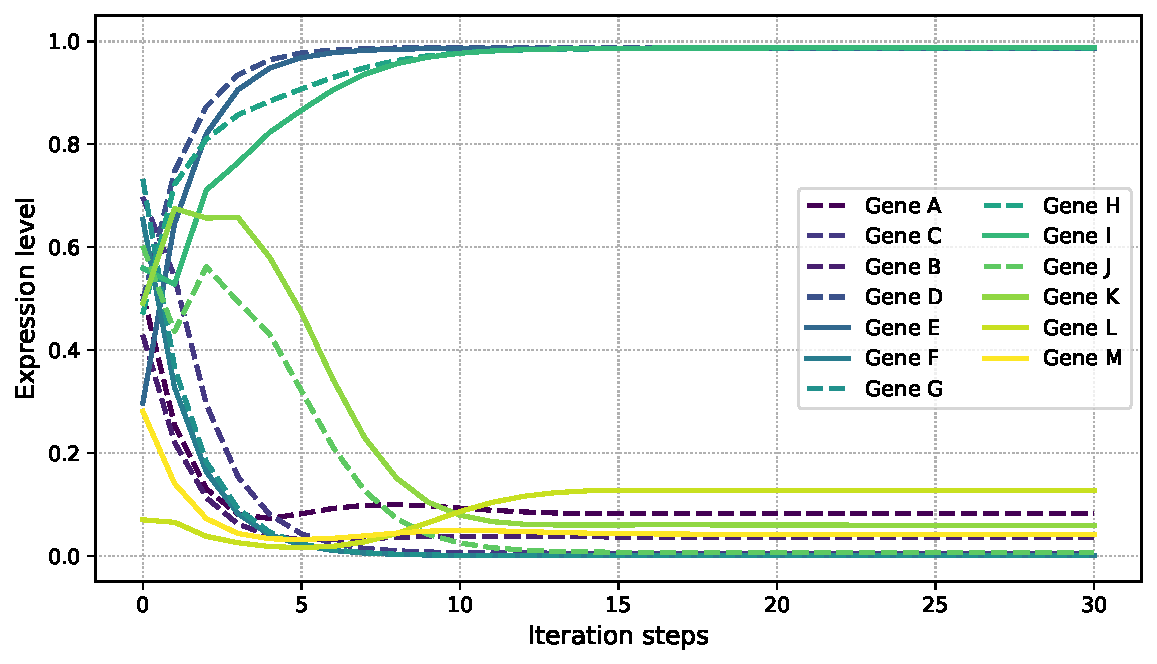
\includegraphics[width=\textwidth]{alife/img/inversion_expr_level.pdf}
\label{subfig:alife:inversion_expr}
\end{subfigure}
\caption[Effect of a genomic inversion on the example individual in Figure~\ref{fig:alife:13genes}]{Genome, local supercoiling and gene expression levels of a new individual obtained from the individual in Figure~\ref{fig:alife:13genes} by switching the positions and orientations of genes B and C.}
\label{fig:alife:inversion}
\end{figure}

Figure~\ref{fig:alife:inversion} again shows the local supercoiling and gene expression levels of the individual in Figure~\ref{fig:alife:13genes}, after reversing the positions and orientations of genes B and C.
This is an example of a genomic inversion, which will be presented in further detail in section~\ref{sec:inversion}.
The starting point of this inversion falls between genes A and B and its end point between genes C and D; this results in the reversal of segment [BC] relative to the rest of the genome.
Here, we can see that the diverging orientation that was present between genes A and B has vanished, replaced by a set of genes in colinear orientation, from A to D.
This genomic reorganization results in the loss of the activation of genes A and B, as gene B is now more strongly inhibited by gene D due to its closer genomic location, and as genes A and B are not in a positive feedback loop -- due to diverging orientations -- any longer; only the pairs of genes D and E, and H and I, remain activated.

Based on these observations, we can confirm that in our model, the transcription"=supercoiling coupling generates complex networks of genome-wide interactions between genes, and that these networks directly depend on the architecture of the genome.


\section{An Evolutionary Genome-Wide Model of the Transcription-Supercoiling Coupling}
\sectionmark{An Evolutionary Genome-Wide Model of the TSC}
\label{sec:alife:evol_model}

After evidencing that transcriptional activity depends on the organization of the genome, we now question to which extent evolution can simultaneously leverage the organization of the genome and the transcription-supercoiling coupling in order to adapt gene regulatory activity to different environments.
Indeed, as has been observed in \emph{Dickeya dadantii}~\citep{muskhelishvili2019}, different phenotypes can evolve as a response to different supercoiling levels induced by the environment, and the transcription-supercoiling coupling could play a role in enabling the existence of this reaction norm.

In this section, we expand our model into an evolutionary simulation.
At each generation of the simulation, all individuals are evaluated and their fitness values are computed, based on their gene transcription levels.
Then, the individuals of the new generation are chosen by picking their ancestor from the current generation, with a probability proportional to the ancestor's fitness.
The model is panmictic, meaning that any individual in the population can be chosen as the ancestor of any new individual.
Finally, during replication, the genome of each new individual stochastically undergoes a number of mutations, before the new individual is evaluated again; importantly, these mutations do not impact genes themselves, but only the spatial organization of the genome: gene orientations, syntenies, and intergenic distances.

\subsection{Evolutionary Model: Evolution in Two Separate Environments}

We model the evolution of populations of individuals that experience two different environments, named A and B.
Each environment is defined by its value of $\sigma_{env}$, respectively $\sigma_A$ and $\sigma_B$, which represent the change in the supercoiling level due to the environment~\citep{dorman2016}.
In order to have environments with distinct effects, we choose a value of $\sigma_A = 0.1$, for which isolated genes are effectively inhibited (as in the top-left panel of Figure~\ref{fig:alife:sigma_env}), and a value of $\sigma_B = -0.1$, for which some but not all genes are activated (bottom-left panel).

We separate genes into three classes, based on the environments in which they must be activated: either in both environment A and environment B (\emph{AB} genes), only in environment A (\emph{A} genes), or only in environment B (\emph{B} genes).
These classes allow us to define optimal phenotypes for both environments: in environment A, both \emph{A} and \emph{AB} genes should be activated, whereas \emph{B} genes should be inhibited.
Conversely, in environment B, only \emph{B} and \emph{AB} genes should be activated, but not \emph{A} genes.


\subsection{Fitness}

In order to compute the fitness of an individual, we define an optimal phenotype $\tilde{e}^A$ (resp. $\tilde{e}^B$), corresponding to the vector of the expected expression level $\tilde{e}^A_i$ for each gene $i$ in environment A (resp. environment B).
We choose an expected expression level of $\tilde{e} = 1$ for genes that should be activated, which corresponds to the maximum possible expression level of a gene in our model.
Similarly, we choose $\tilde{e} = 0$ for genes that should be inhibited, which is the minimum expression level that is attainable.
Then, in each environment, we compute the gap $g_A$ (resp. $g_B$), or average square distance of the individual's gene transcription levels $e^A$ (the vector constituted by the transcription level $e^A_i$ of each gene $i$) to the optimal levels $\tilde{e}^A$ (resp. $e^B$ and $\tilde{e}^B$).
The gap $g_A$ is computed as follows:

\begin{equation}
g_A(e^A) = \frac{1}{n} \sum_{i=1}^{n} (e^A_i - \tilde{e}^A_i)^2
\label{eq:alife_gap}
\end{equation}

The gap $g_B$ is computed in the same way.
Finally, we compute the fitness of the individual by summing the gap in each environment, and applying an exponential scaling: $f = e^{-k (g_A + g_B)}$, where $k$ is a scaling factor representing the selection pressure.
A higher value of $k$ means that well-adapted individuals, those which have a smaller gap, will have an even higher fitness value compared to other individuals; we typically use $k=50$, meaning that a small decrease in the gap compared to other individuals yields a large reproductive advantage.


\subsection{Mutational Operator: Genomic Inversions}
\label{sec:inversion}

We introduce only one kind of mutation in our model, which is genomic inversions: we choose two breakpoints randomly on the genome, and reverse the genomic content between these points.
Genes are then reinserted in the genome in the opposite orientation and order, taking care to update all intergenic distances appropriately.
Note that in our model, genes have a length of zero and the breakpoints can therefore not fall inside a gene.
Moreover, an inversion has no effect if both breakpoints fall between two neighboring genes (as only an intergenic region would be affected), but can impact any number of genes otherwise.
Genomic inversions hence affect gene syntenies and orientations, and therefore affect gene expression levels as presented in subsection~\ref{sec:alife:gene_pos}.
When mutating a genome during reproduction, we draw the number of inversions $k$ to perform from a Poisson law with parameter $\lambda = 2$, giving an average of 2 inversions between an individual and its ancestor; the probability of not undergoing any mutations is $P(k=0) = e^{-\lambda} \approx 0.136$.

\begin{figure}[H]
\centering
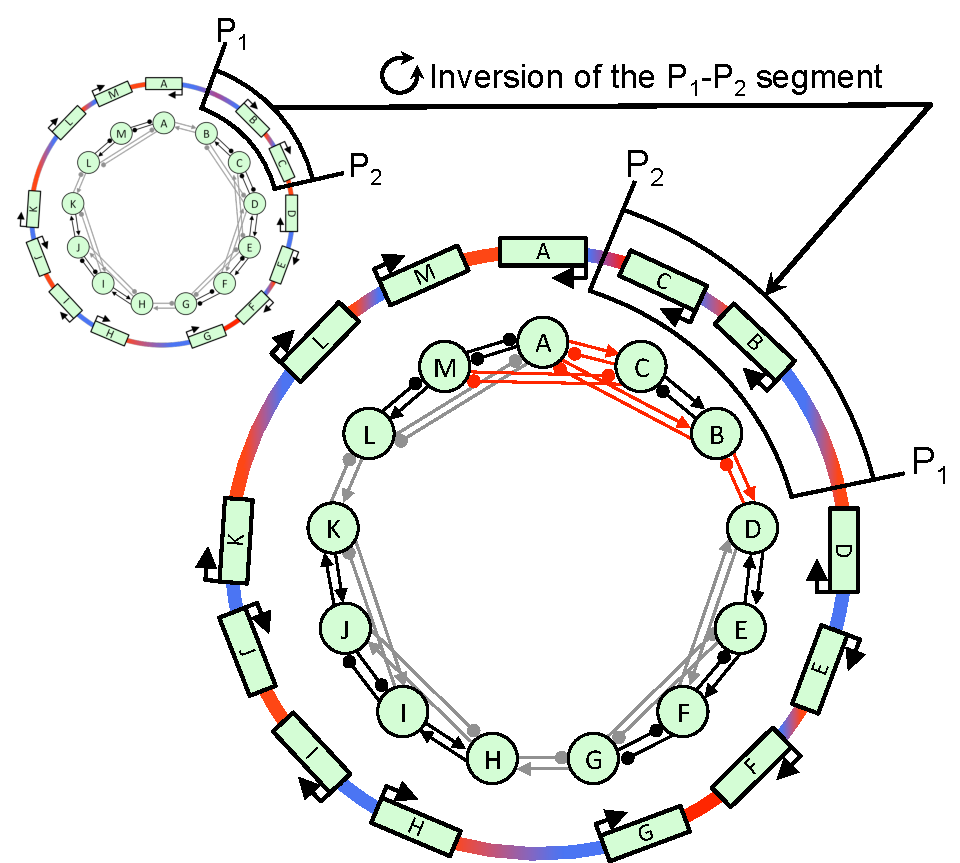
\includegraphics[width=0.8\textwidth]{alife/img/genome_inversion.pdf}
\caption[Effect of an inversion on the hand-drawn genome in Figure \ref{fig:alife:network}]{Result of the inversion of a genomic segment containing genes B and C from the individual presented in Figure~\ref{fig:alife:network}.
The gene interactions which have changed due to the inversion are drawn in red.
This illustration genome corresponds to the actual individual in our model presented in Figure~\ref{fig:alife:inversion}.}
\label{fig:alife:genome_inv}
\end{figure}

Figure \ref{fig:alife:genome_inv} presents a genome obtained by performing an inversion on the genome shown in Figure~\ref{fig:alife:network}.
As a result of this inversion, genes B and C have been switched from the forward to the backward orientation, and the intergenic distances between A and C on the one hand, and B and D on the other hand, have been modified; however, the relative orientation of B and C, and hence their interaction subnetwork, remain unchanged.
This results in changes to the gene interaction network: instead of mutual activation between genes A and B and mutual inhibition between genes C and D, all four genes now lie in colinear orientations, in which each of these genes activates its upstream neighbor but represses its downstream neighbor.

\subsection{Experimental Setup and Parameter Values}

We initialized the simulation with a clonal population of $N=100$ copies of an initial individual with the following genome: 60 genes in random orientations, uniformly distributed along a 60,000 bp genome, and equally divided between the \emph{AB}, \emph{A} and \emph{B} classes.
We chose a maximum interaction distance of $d_{max} = 2500$, meaning that each gene initially interacts with its 2 closest neighbors in each direction through the transcription-supercoiling coupling.
Note that as inversions may change intergenic distances, genes can move closer or further apart during evolution.
We set the basal supercoiling level $\sigma_{basal}$ to the average supercoiling level in \emph{E. coli} of -0.06~\citep{crozat2005}, and $\sigma_0$ to $-0.06$ as well, so that in the absence of other sources of supercoiling (either environmental or through the coupling), the default activity level of a gene is 0.5.
Finally, we set $c = 0.3$, in order to have comparable values for the variations in supercoiling due to the environment and due to the transcription-supercoiling coupling, and $\epsilon=0.03$, so that the variations in supercoiling have a qualitatively mild effect on gene expression.


In order to run the simulations, we evolved 15 different populations for 250,000 generations; the simulation lasted for approximately 48h on a computer with Intel Xeon E5-2640 v3 @ 2.60GHz CPUs, using around 100 MB of RAM per replicate.


\subsection{Adaptation of Gene Expression Levels to Different Environments}

Figure~\ref{fig:alife:mean_activ} summarizes the differences in the proportion of activated genes for each of the three sets of genes, between environments A and B, averaged over the 15 repetitions.
In the figure, we consider a gene to be activated if its activity at the end of the lifecycle is over $0.5$, and we look at the average proportion of activated genes in the best individual of every replica.
Let us recall that the evolutionary target for \emph{AB} genes is an expression level of 1 in both environments, for \emph{A} genes an expression level of 1 in environment \emph{A} and 0 in \emph{B}, and vice-versa for \emph{B} genes.
After 250,000 generations of evolution, individuals have acquired genomes that allow all \emph{AB} genes to be activated in both environments, and that allow all \emph{B} genes to be activated in environment B and inhibited in environment A.
On average, over 60\% of \emph{A} genes are activated in environment A, which imposes a positive change in supercoiling ($\sigma_A = 0.1$) and makes gene activation harder.
Conversely, less than 5\% of \emph{A} genes are activated in environment B, in which gene activation is easier ($\sigma_B = -0.1$).
The final expression levels of \emph{A} genes therefore show that specific sets of genes can be activated by the transcription-supercoiling coupling despite environmental hurdles.

\begin{figure}[H]
\centering
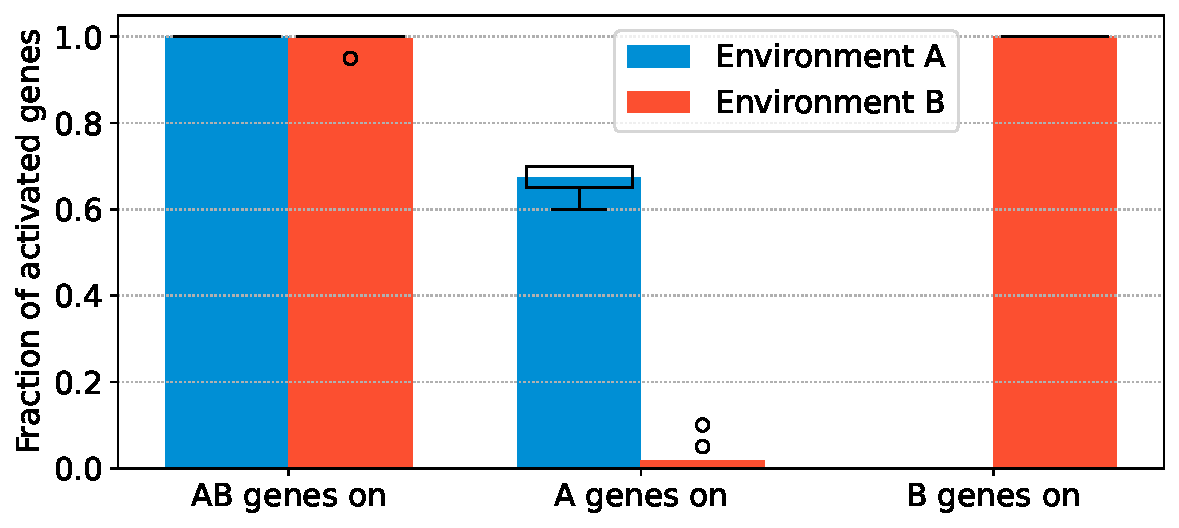
\includegraphics[width=0.8\textwidth]{alife/img/mean_activation.pdf}
\caption[Fraction of activated genes of each type at the end of evolution in the proof-of-concept model]{Fraction of activated genes of each type in each environment at the end of the lifecycle, averaged over the best individuals in the last generation of each replica.
The boxplots represent the median and quartiles, and the dots flier data points.
For \emph{A} genes and \emph{B} genes, activation levels differ depending on the environment: $p$-value $2.40\times10^{-17}$ for \emph{A} genes, and $p$-value $<1\times10^{-25}$ for \emph{B} genes (Student's $t$-test for dependent samples).}
\label{fig:alife:mean_activ}
\end{figure}

Furthermore, in each of the 15 replicates, the fitness of the best individual in the population increases continuously over the course of evolution, as shown in Figure~\ref{fig:alife:fitnesses}.
As their respective fitness keeps increasing until the end of the simulation, this suggests that fitter phenotypes remain reachable through further evolution by genomic rearrangements.
The rhythm of evolution is however progressively slower and slower (note the logarithmic time scale in the figure), as the pool of available favorable mutations decreases.

\begin{figure}[H]
\centering
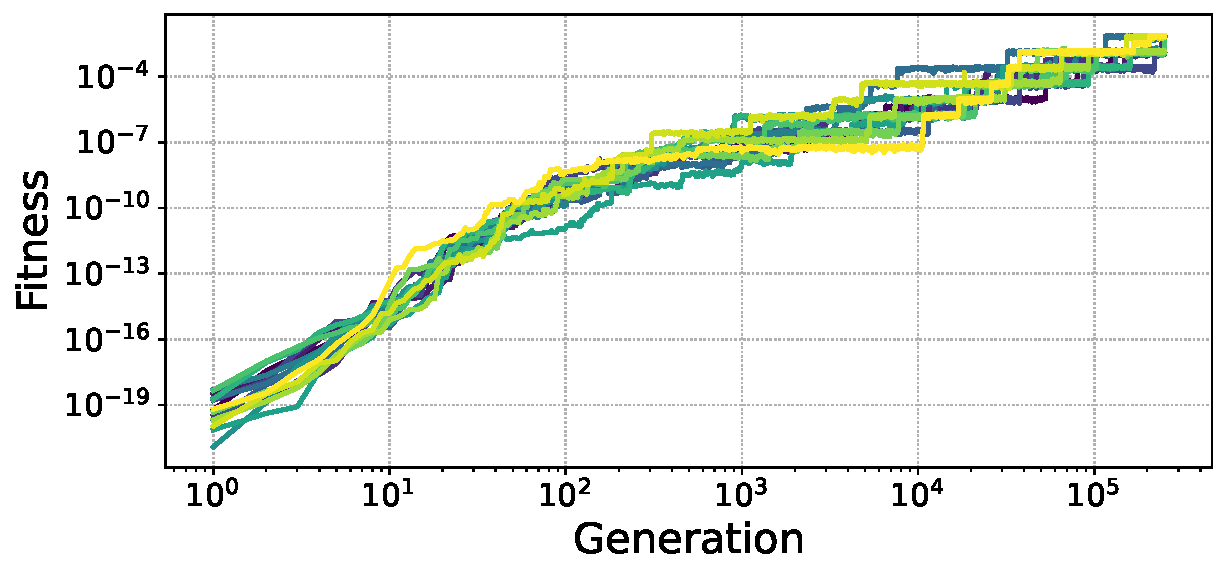
\includegraphics[width=0.8\textwidth]{alife/img/all_fitness.pdf}
\caption[Fitness of every replicate during evolution in the proof-of-concept model]{Evolution of the fitness of the best individual of each replicate at every generation.}
\label{fig:alife:fitnesses}
\end{figure}

Finally, details of the evolution of one of the 15 replicate populations are shown in Figure~\ref{fig:alife:evolution}.
We can first see that the number of activated \emph{AB} genes of the best individual at each generation quickly rises to 20 (out of 20 genes of that type) in both environment A and environment B; this shows that evolving a phenotype that is resistant to environmental perturbations, having genes that are always activated, is easy in the model.
For \emph{A} genes and \emph{B} genes, we observe an asymmetric tendency during the course of evolution towards activation in the target environment, and inhibition in the opposite environment.
However, the difference in the number of activated \emph{B} genes between environment A and environment B is much higher than for \emph{A} genes.
As already mentioned above, this asymmetry comes from the different requirements expected of \emph{A} genes and \emph{B} genes: gene activation is easier in environment B than in environment A, as it is easier for a gene to become activated in an environment with a lower overall supercoiling level.
\emph{A} genes therefore have to be activated in a harder environment, and inhibited in a simpler environment, whereas \emph{B} genes have to do the opposite.

\begin{figure}[H]
\centering
\begin{subfigure}[t]{0.8\textwidth}
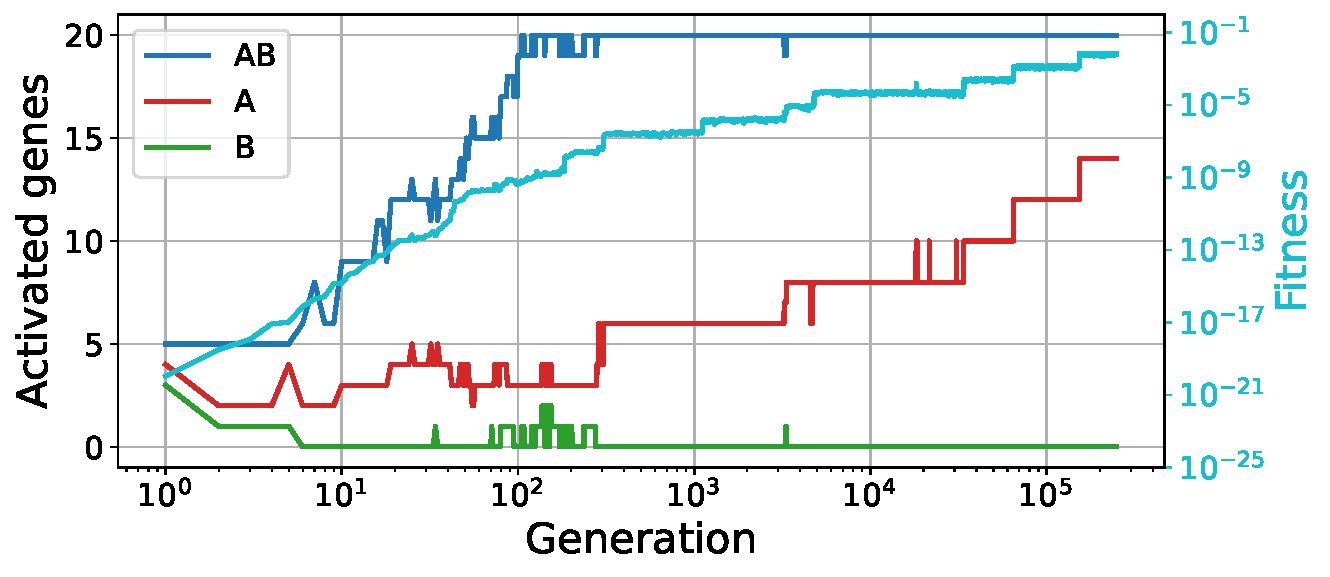
\includegraphics[width=\textwidth]{alife/img/rep_13_env_A.pdf}
\label{subfig:alife:env_A}
\end{subfigure}

\begin{subfigure}[t]{0.8\textwidth}
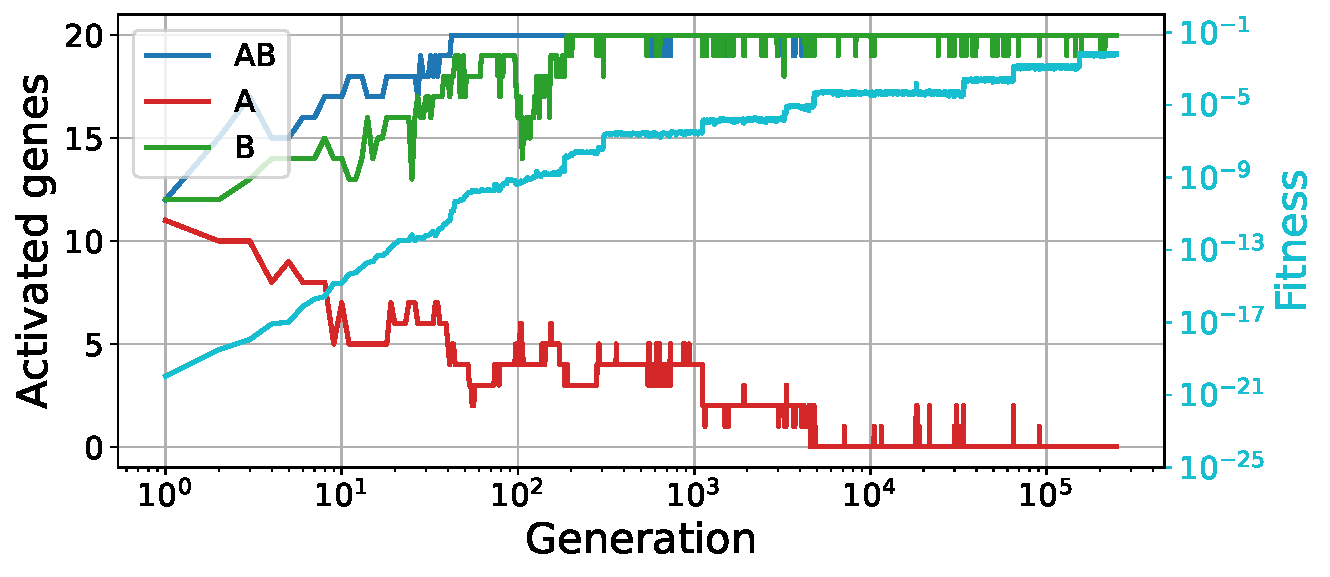
\includegraphics[width=\textwidth]{alife/img/rep_13_env_B.pdf}
\label{subfig:alife:env_B}
\end{subfigure}

\caption[Number of activated genes during evolution in one of the replicates in the proof-of-concept model]{Number of activated genes of each type and fitness of the best individual at every generation of replicate 13, with a population size of $N=100$, for 250,000 generations.
The number of active \emph{AB} genes increases until it reaches 20, in both environment A (top) and environment B (bottom).
The number of active \emph{A} (resp. \emph{B}) genes increases in environment A (resp. B) and decreases in environment B (resp. A) over time, thus converging towards their evolutionary target.}
\label{fig:alife:evolution}
\end{figure}

This is shown in more detail in Figure~\ref{fig:alife:best_indiv}, which shows the supercoiling level and gene activation levels of the best individual of the last generation of replicate 13, in both environments.
The phenotypes displayed in each environment present clearly distinct gene expression patterns.
In environment A (top), nearly all genes converge directly towards their final state, whereas in environment B (bottom), most \emph{A} genes (in red) and some \emph{B} genes (in green) show a complex trajectory of activation levels before reaching their stable state.
Moreover, genomic domains with markedly different supercoiling levels emerge through the transcription-supercoiling coupling, with both very overwound and very underwound zones.
These domains also show qualitatively different responses to different environments: in some domains, the supercoiling level is very similar (around gene 0, gene 15 or gene 55 for example), while in others supercoiling is completely different in each environment (between genes 20 and 35).
This shows the plasticity of the response to environmental change at the local supercoiling level.

\begin{figure}[H]
\centering
\begin{subfigure}[t]{0.42\textwidth}
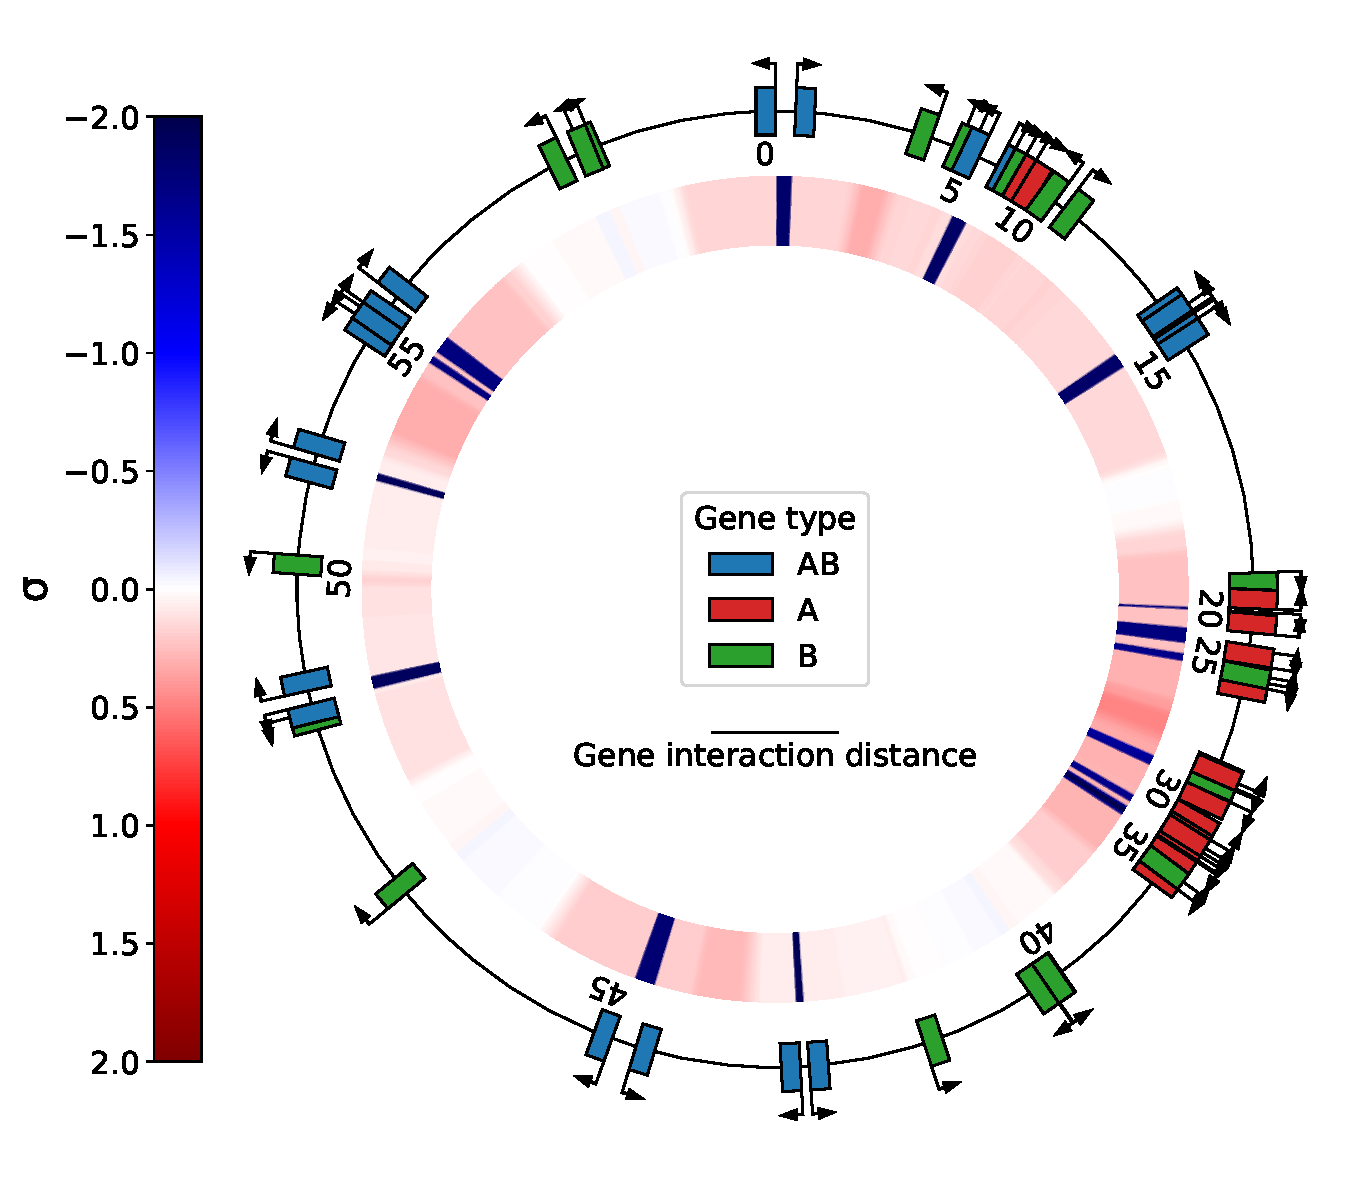
\includegraphics[width=\textwidth]{alife/img/genome_and_tsc_rep13_env_A.pdf}
\label{subfig:alife:best_genome_A}
\end{subfigure}
\begin{subfigure}[t]{0.56\textwidth}
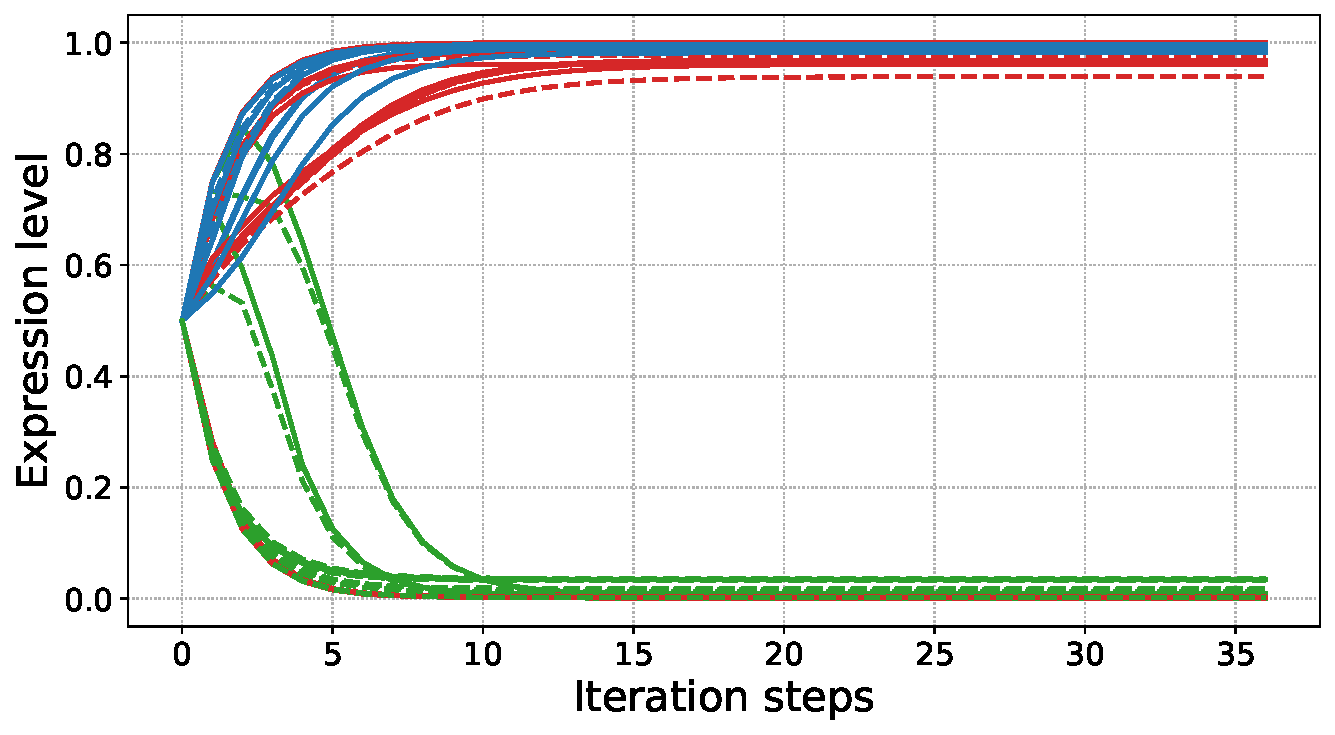
\includegraphics[width=\textwidth]{alife/img/best_rep13_env_A.pdf}
\label{subfig:alife:best_expr_A}
\end{subfigure}
\vspace{-5mm}

\begin{subfigure}[t]{0.42\textwidth}
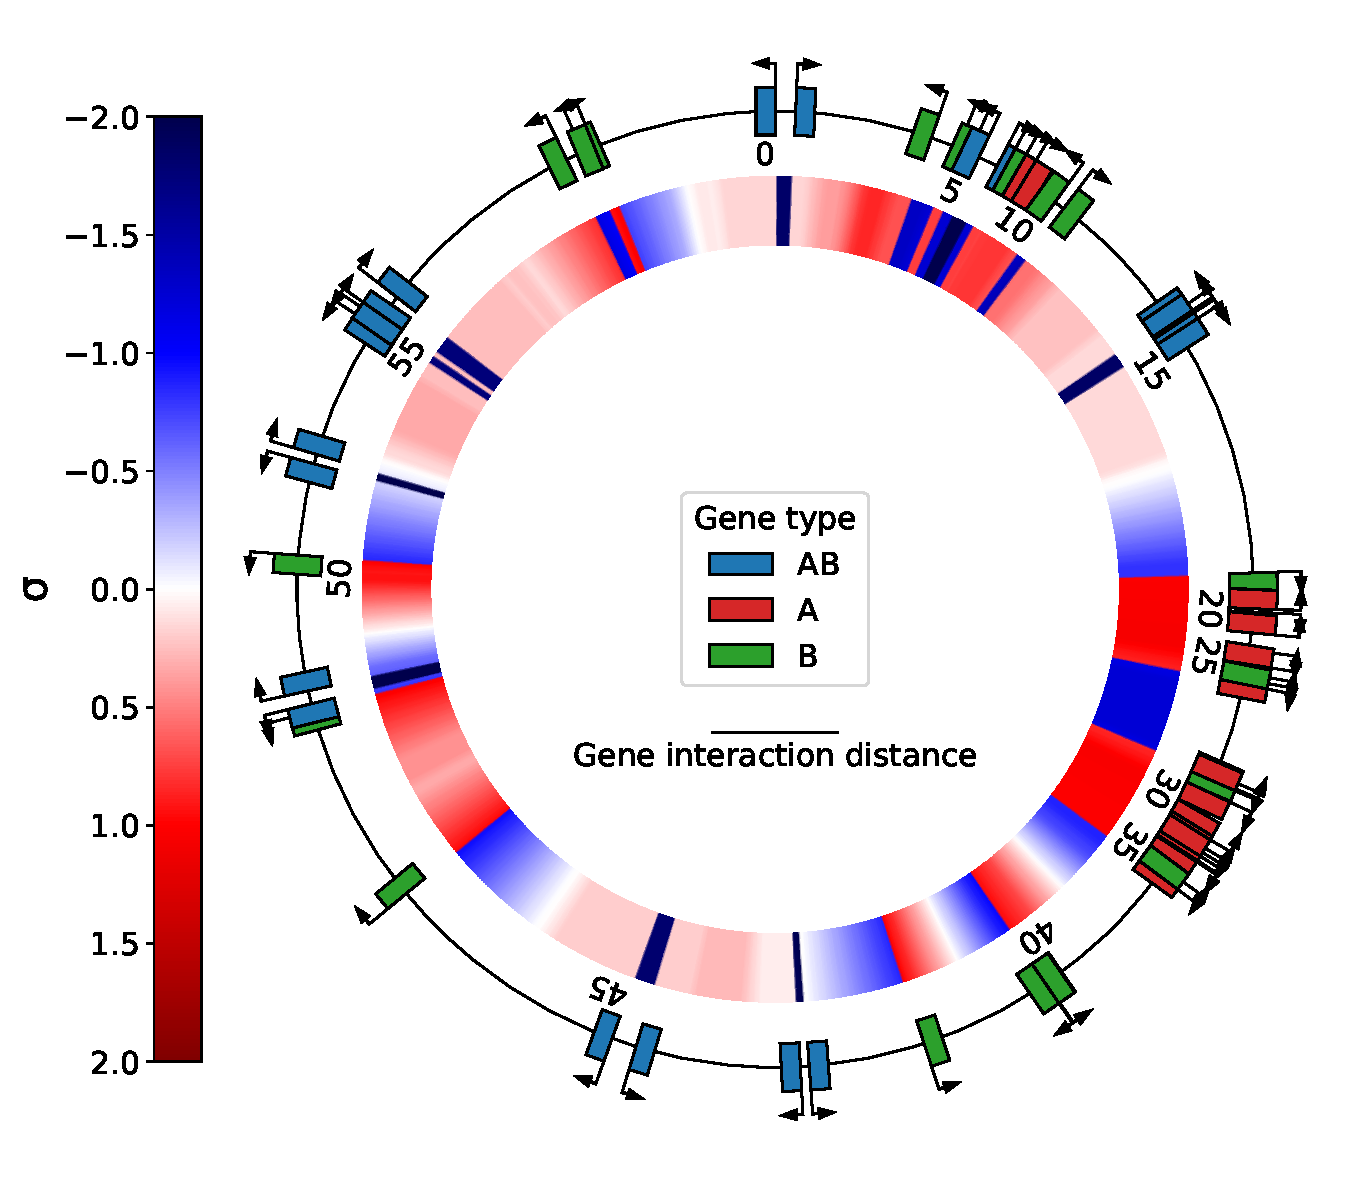
\includegraphics[width=\textwidth]{alife/img/genome_and_tsc_rep13_env_B.pdf}
\label{subfig:alife:best_genome_B}
\end{subfigure}
\begin{subfigure}[t]{0.56\textwidth}
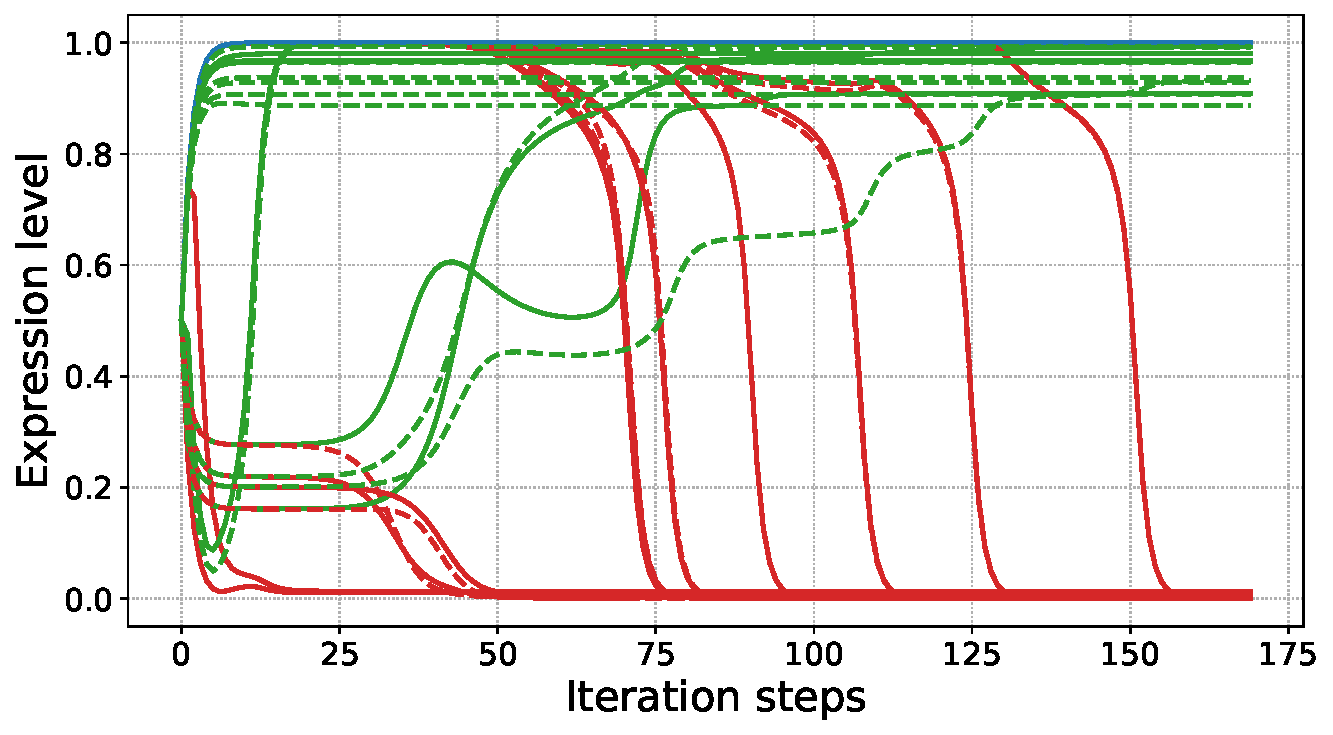
\includegraphics[width=\textwidth]{alife/img/best_rep13_env_B.pdf}
\label{subfig:alife:best_expr_B}
\end{subfigure}
\caption[Best individual at the end of evolution in one of the replicates in the proof-of-concept model, evaluated in both environments]{Local supercoiling along the genome and gene transcription levels of the best individual in replicate 13 after 250,000 generations.
Environment A is on top and environment B at the bottom.
\emph{AB} genes are colored blue, \emph{A} genes colored red, and \emph{B} genes colored green.}
\label{fig:alife:best_indiv}
\end{figure}

Our experimental results show that, in a model of gene transcription that is structured around the transcription"=supercoiling coupling, complex gene interaction networks can in fact evolve.
These gene interaction networks are sensitive to environmental variations, which are mediated in our model by a single parameter: $\sigma_{env}$, the amount of global supercoiling that is due to the environment.

\subsection{Robustness of Gene Network Evolution}
\label{sec:alife:param_explor}

In order to ensure that our results remain experimentally valid over a broad range of parameter values, we ran additional sets of simulations.
We changed respectively the sensitivity of gene promoters to supercoiling changes ($\epsilon$ in equation~\ref{eq:transcr}), the interaction coefficient used in computing the local supercoiling due to the transcription-supercoiling coupling ($c$ in equation~\ref{eq:dsde}), and the strength of the change in supercoiling imposed by the environment ($\sigma_A$ and $\sigma_B$).
We chose sets of logarithmically-spaced values for each parameter, and ran 5 replicates of the evolution experiment for 250,000 generations for each parameter value.
Note that, for extreme parameter values, gene expression levels did in some cases not converge to stable states by the maximum number of computation steps.
In this situation, we chose to retain the gene expression levels at the last step as the phenotype of the affected individuals.

\begin{figure}[H]
\centering
\begin{subfigure}[t]{0.49\textwidth}
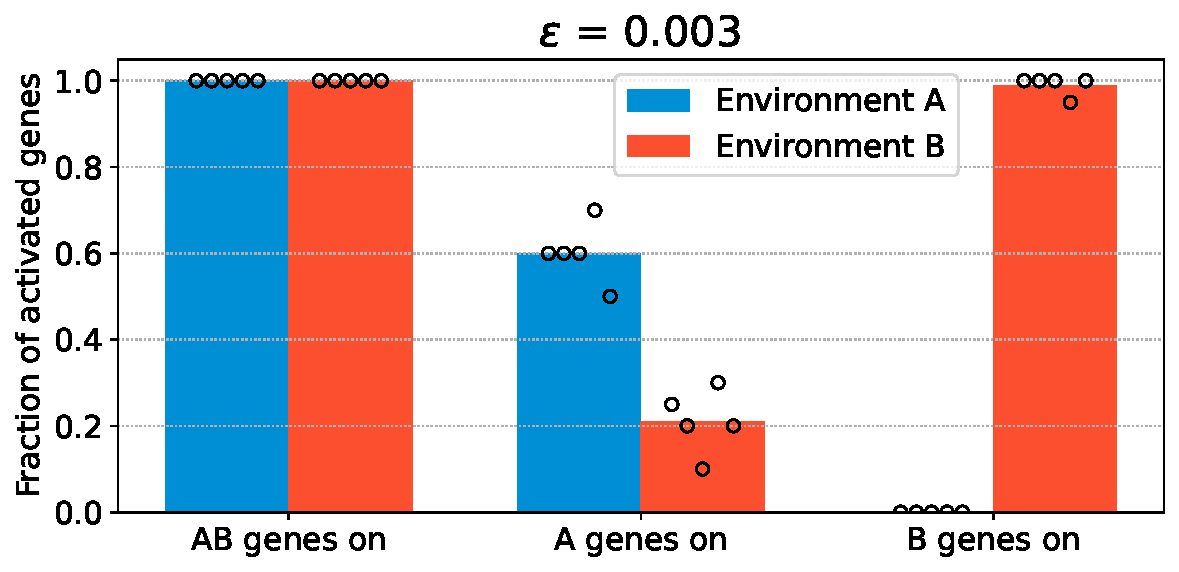
\includegraphics[width=\textwidth]{alife/img/mean_activation_epsilon-0.003.pdf}
\label{subfig:alife:param_epsilon_1}
\end{subfigure}
\begin{subfigure}[t]{0.49\textwidth}
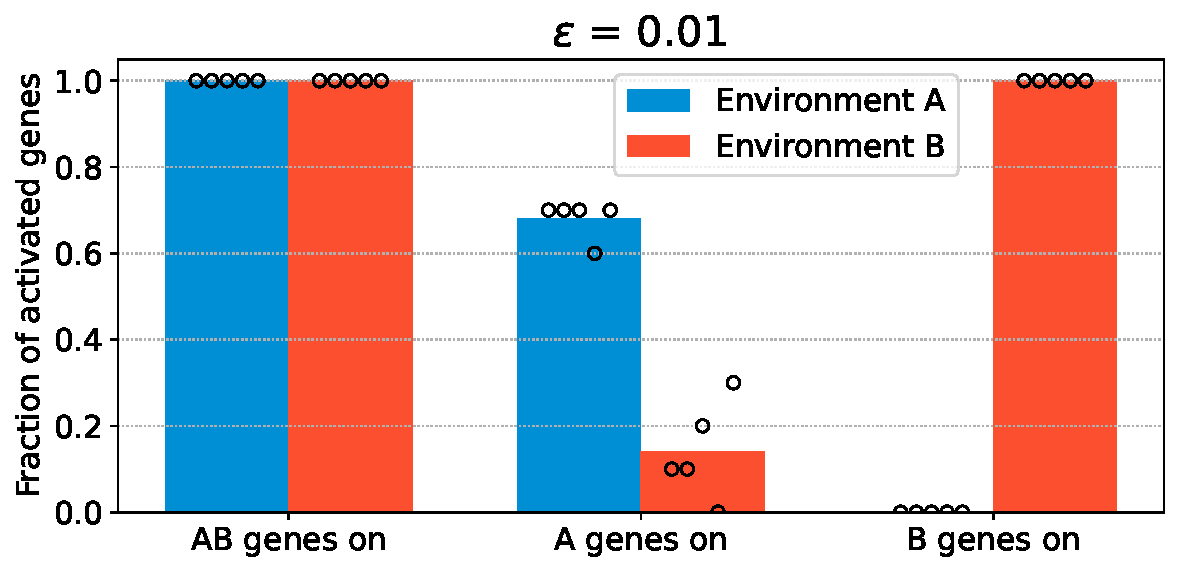
\includegraphics[width=\textwidth]{alife/img/mean_activation_epsilon-0.01.pdf}
\label{subfig:alife:param_epsilon_2}
\end{subfigure}

\begin{subfigure}[t]{0.49\textwidth}
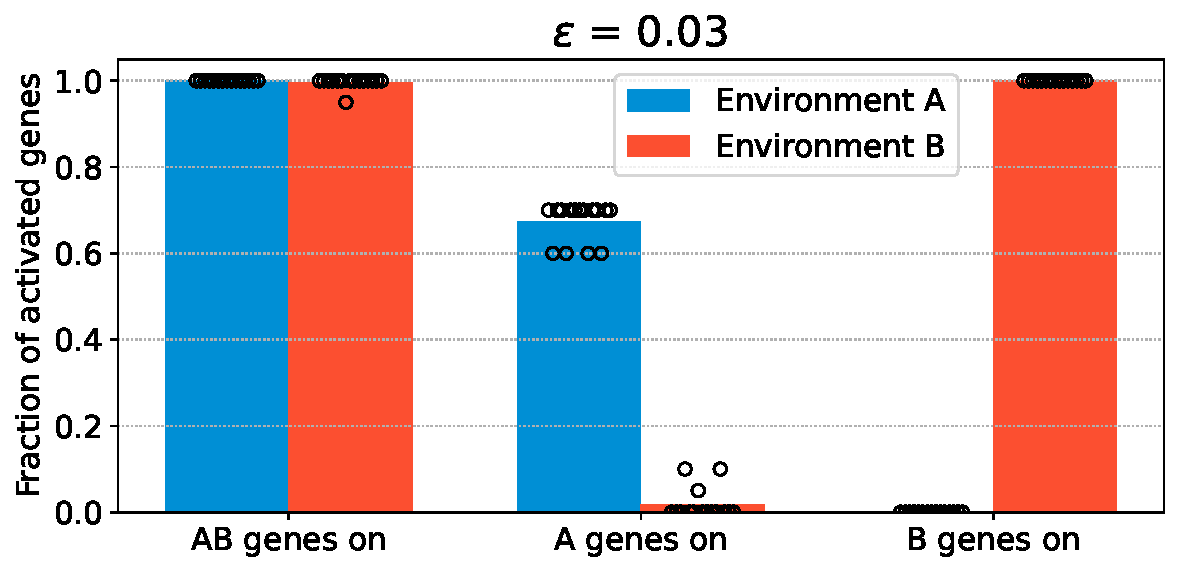
\includegraphics[width=\textwidth]{alife/img/mean_activation_epsilon.pdf}
\label{subfig:alife:param_epsilon_3}
\end{subfigure}
\begin{subfigure}[t]{0.49\textwidth}
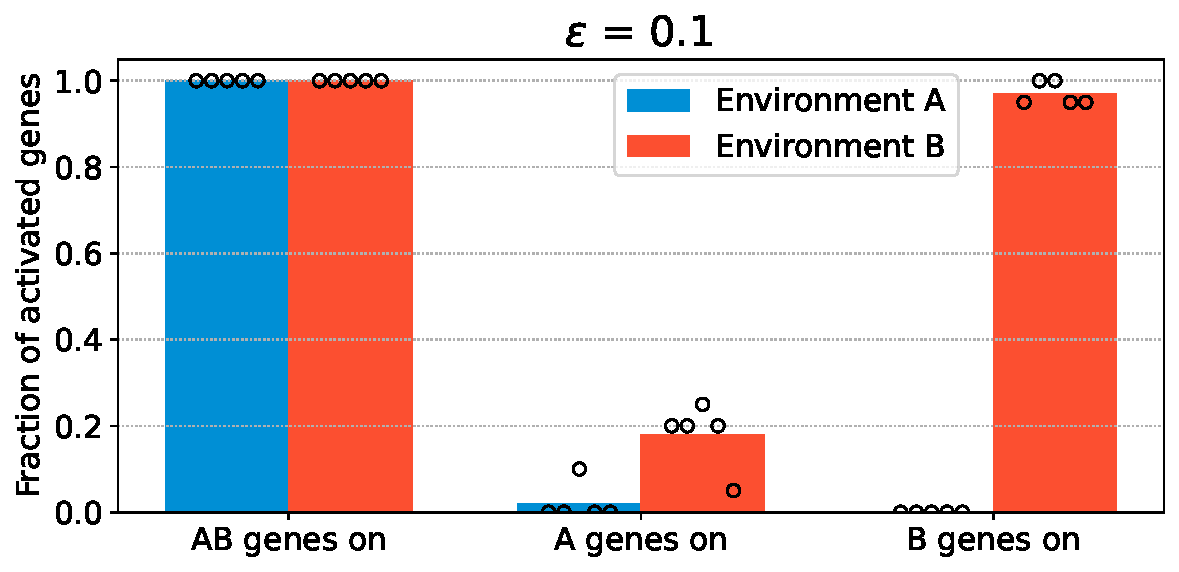
\includegraphics[width=\textwidth]{alife/img/mean_activation_epsilon-0.1.pdf}
\label{subfig:alife:param_epsilon_4}
\end{subfigure}
\caption[Parameter exploration in the proof-of-concept model: varying $\epsilon$]{Average fraction of activated genes in each environment at the end of evolution, for increasing values of $\epsilon$, from top to bottom and left to right.
Every replicate is shown as a dot, and the bottom-left panel ($\epsilon = 0.03$) recalls data from the main run (which has 15 replicates) for comparison.
For all values of $\epsilon$ except $0.1$, the behavior from the main run is qualitatively replicated.}
\label{fig:alife:param_epsilon}
\end{figure}

The results of these additional simulations are presented in figures~\ref{fig:alife:param_epsilon},~\ref{fig:alife:param_c} and~\ref{fig:alife:param_sigma}.
For $\epsilon$, we chose values of $\epsilon = 0.003$, $\epsilon = 0.01$, and $\epsilon = 0.1$, compared to an initial value of $\epsilon = 0.03$, and the results are shown in Figure~\ref{fig:alife:param_epsilon}.
For the values of $\epsilon$ lower than the default (top row), representing a higher sensitivity of promoters to supercoiling, we observe the evolution of differentiated gene expression levels as in the main run (bottom-left panel), whereas for the higher value of $\epsilon$ (bottom-right panel), \emph{A} genes are still not expressed in environment A by the end of evolution.
In this case, promoters are not sensitive enough to the supercoiling variations caused by the transcription-supercoiling coupling, and genes are unable to overcome the highly positive supercoiling of environment A.

\begin{figure}[H]
\centering
\begin{subfigure}[t]{0.49\textwidth}
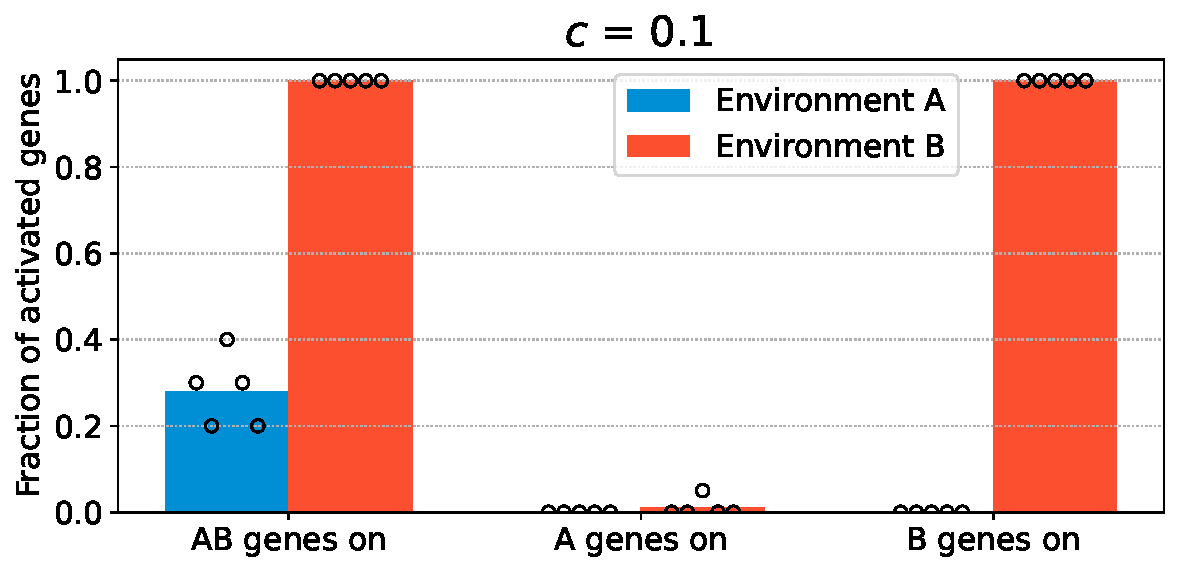
\includegraphics[width=\textwidth]{alife/img/mean_activation_inter-coef-0.1.pdf}
\label{subfig:alife:param_c_1}
\end{subfigure}
\begin{subfigure}[t]{0.49\textwidth}
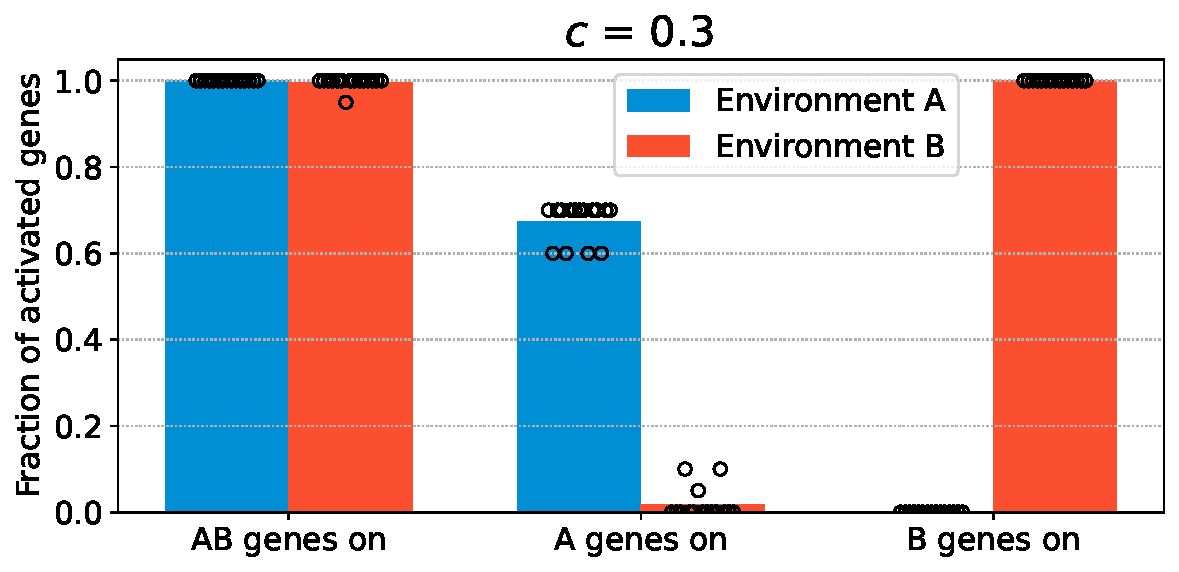
\includegraphics[width=\textwidth]{alife/img/mean_activation_inter_coef.pdf}
\label{subfig:alife:param_c_2}
\end{subfigure}

\begin{subfigure}[t]{0.49\textwidth}
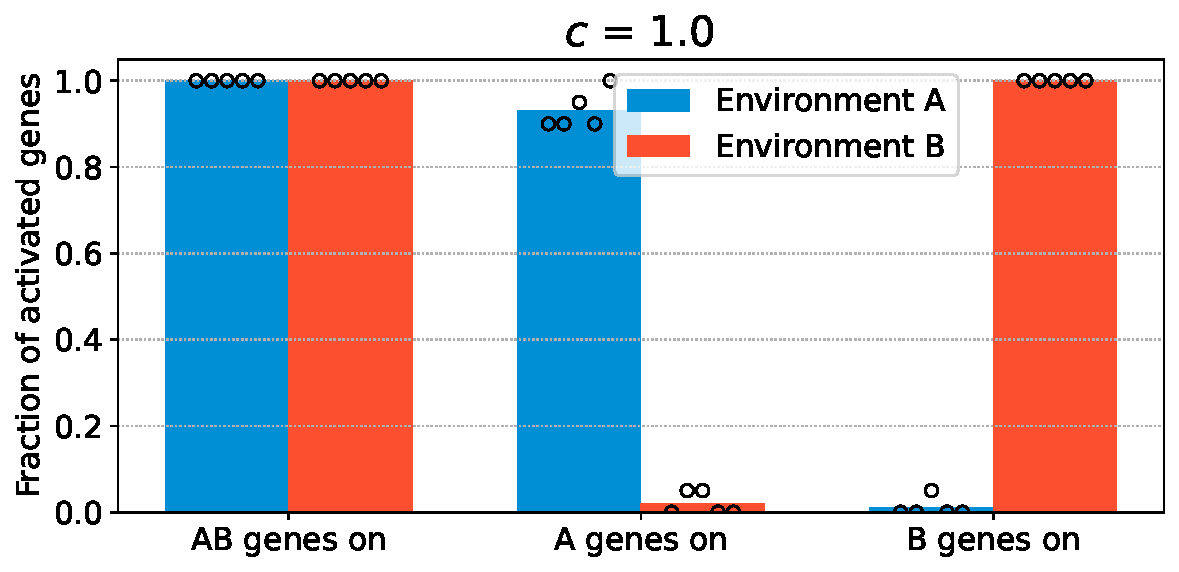
\includegraphics[width=\textwidth]{alife/img/mean_activation_inter-coef-1.0.pdf}
\label{subfig:alife:param_c_3}
\end{subfigure}
\begin{subfigure}[t]{0.49\textwidth}
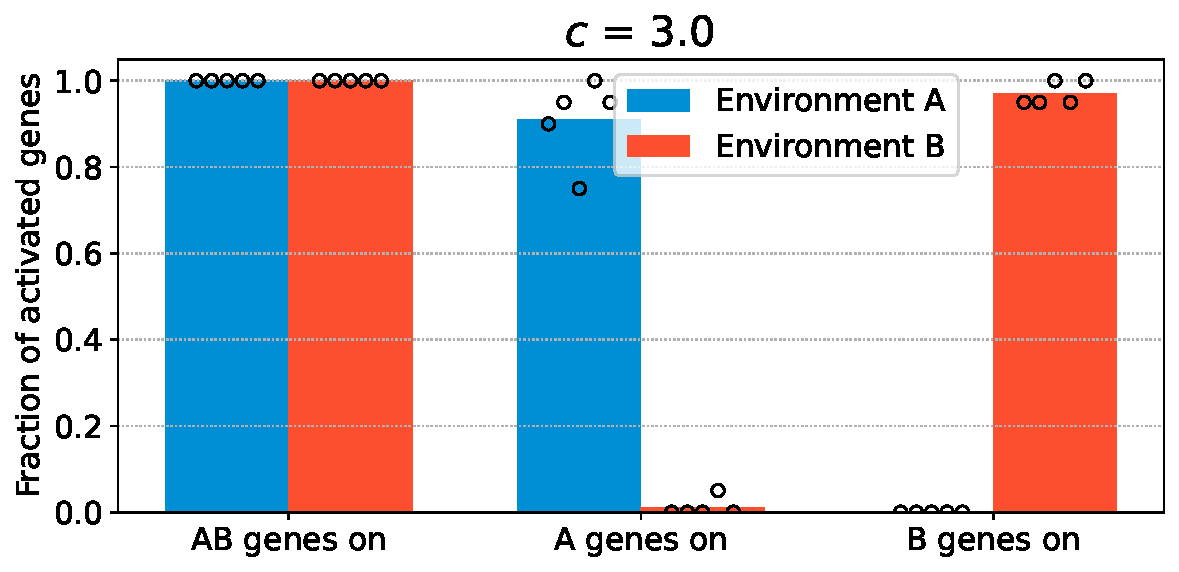
\includegraphics[width=\textwidth]{alife/img/mean_activation_inter-coef-3.0.pdf}
\label{subfig:alife:param_c_4}
\end{subfigure}
\caption[Parameter exploration in the proof-of-concept model: varying $c$]{Average fraction of activated genes in each environment at the end of evolution, for increasing values of $c$, from top to bottom and left to right.
Every replicate is shown as a dot, and the top-right panel ($c = 0.3$) recalls data from the main run for comparison.
For all values of $c$ except $0.1$, the behavior from the main run is qualitatively replicated.}
\label{fig:alife:param_c}
\end{figure}

For $c$, we chose values of $c = 0.1$, $c = 1.0$, and $c = 3.0$, for an initial value of $c = 0.3$, and the results are shown in Figure~\ref{fig:alife:param_c}.
Similarly to $\epsilon$, when $c$ is too low (top-left panel), genes do not interact strongly enough for a differentiated phenotype to evolve as a function of the environment, whereas higher values of $c$ (bottom row) show the same evolutionary behavior as the main run (top-right panel).

\begin{figure}[H]
\begin{subfigure}[t]{0.49\textwidth}
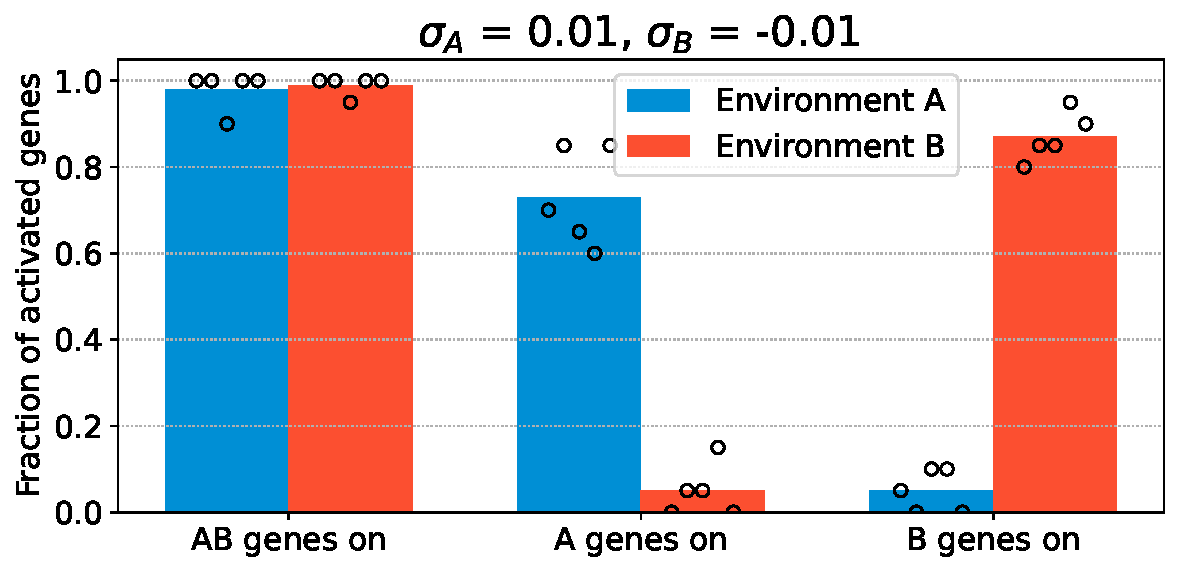
\includegraphics[width=\textwidth]{alife/img/mean_activation_sigma-0.01.pdf}
\label{subfig:alife:param_sigma_1}
\end{subfigure}
\begin{subfigure}[t]{0.49\textwidth}
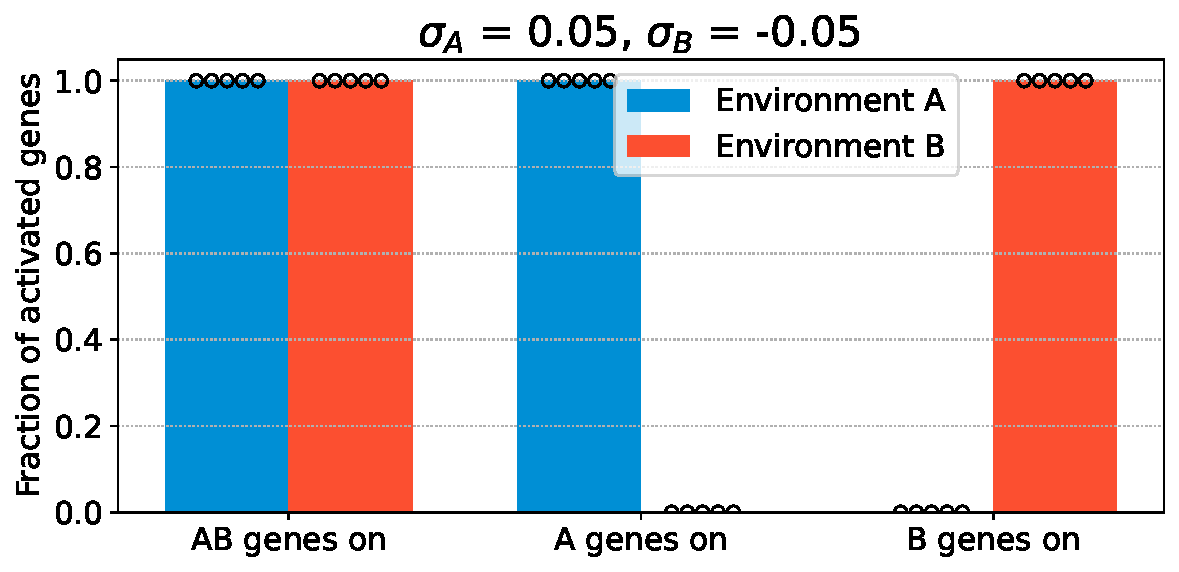
\includegraphics[width=\textwidth]{alife/img/mean_activation_sigma-0.05.pdf}
\label{subfig:alife:param_sigma_2}
\end{subfigure}

\begin{subfigure}[t]{0.49\textwidth}
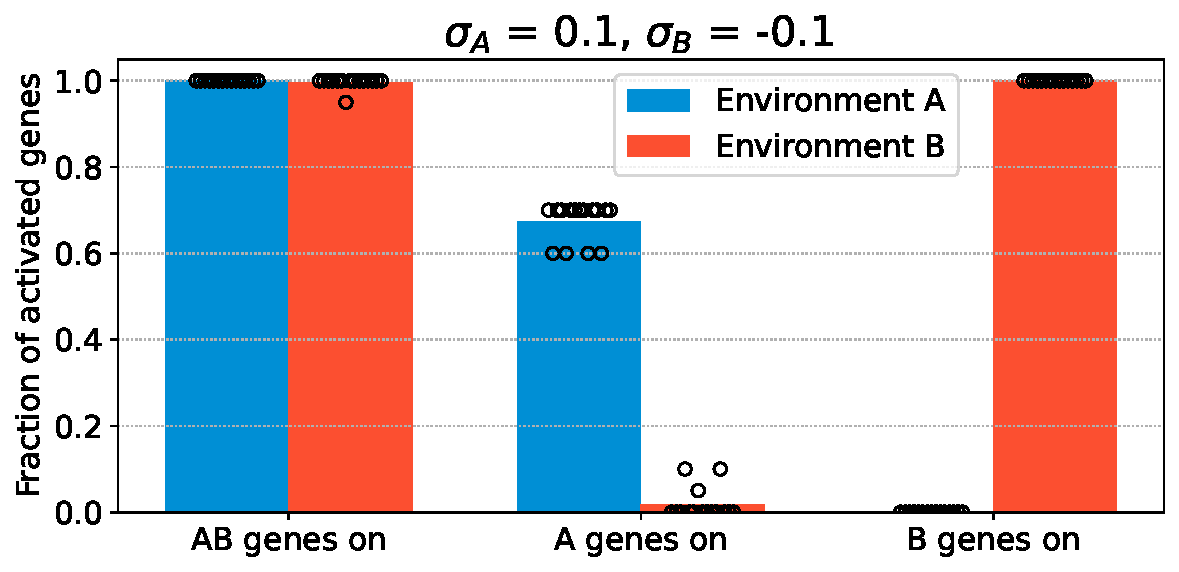
\includegraphics[width=\textwidth]{alife/img/mean_activation_sigma.pdf}
\label{subfig:alife:param_sigma_3}
\end{subfigure}
\begin{subfigure}[t]{0.49\textwidth}
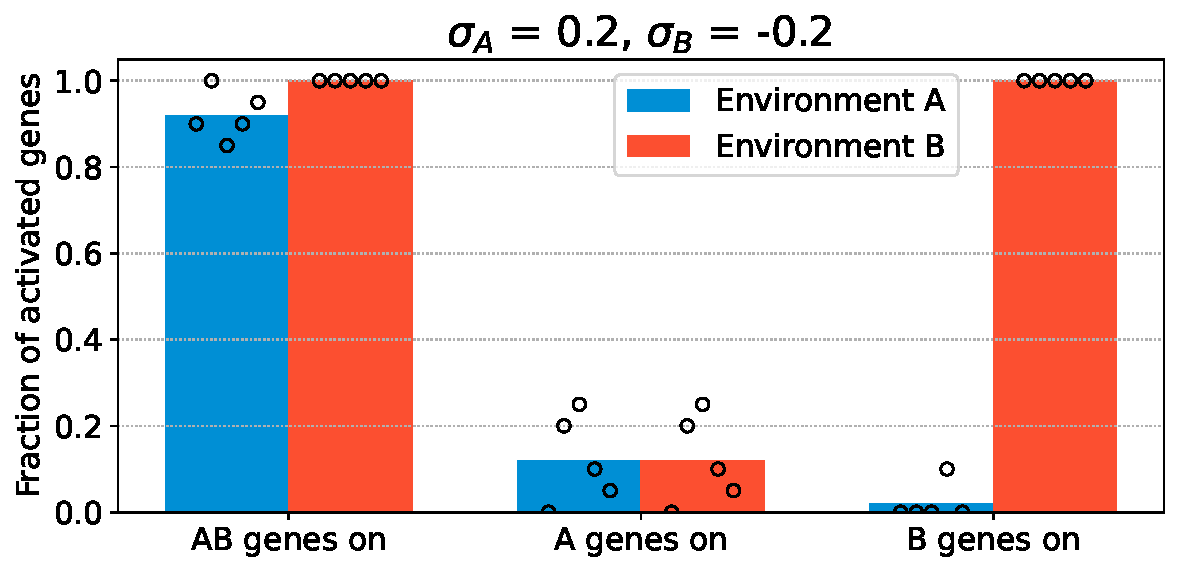
\includegraphics[width=\textwidth]{alife/img/mean_activation_sigma-0.2.pdf}
\label{subfig:alife:param_sigma_4}
\end{subfigure}
\caption[Parameter exploration in the proof-of-concept model: varying $\sigma_A$ and $\sigma_B$]{Average fraction of activated genes in each environment at the end of evolution, for more and more distinct environments $\sigma_A$ and $\sigma_B$, from top to bottom and left to right.
Every replicate is shown as a dot, and the bottom-left panel ($\sigma_A = 0.1$, $\sigma_B = -0.1$) recalls data from the main run for comparison.
For all values except $\sigma_A = 0.2$ and $\sigma_B = -0.2$, the behavior from the main run is qualitatively replicated.}
\label{fig:alife:param_sigma}
\end{figure}

Finally, we also investigate different amplitudes in the difference in supercoiling level between the two environments, by choosing values of $\sigma_A = 0.01$, $\sigma_A = 0.05$ and $\sigma_A = 0.2$, and $\sigma_B = -\sigma_A$ respectively in each case (for an initial value of $\sigma_A = 0.1$ and $\sigma_B = -0.1$).
We observe that, when $\sigma_A = 0.2$ (bottom-right panel), the environmental supercoiling constraint is too high and \emph{A} genes are not activated in environment A by the end of the runs.
However, for environments closer to each other than the default (top row), evolution is able to leverage the differences in supercoiling between these environments to evolve differentiated phenotypes, as in the main run (bottom-left panel), showing that our model remains sensitive to small changes in environmental supercoiling.

To conclude, in our model, the gene interaction network is therefore able to respond to different environments and can evolve an efficient regulation of gene expression under a broad range of parameter values, reinforcing the hypothesis that a supercoiling-mediated coupling between gene expression levels could indeed play a functional role in biological organisms.

\section{Discussion and Perspectives}

DNA supercoiling plays a fundamental role in the regulation of gene transcription in bacteria, and an important part of this role could be mediated by the local variations in supercoiling that are caused by the transcription-supercoiling coupling.
While the influence of the global supercoiling level on gene transcription~\citep{lal2016, ma2016,dorman2016, martisb.2019}, the evolutionary importance of supercoiling regulation~\citep{crozat2005,crozat2010, duprey2021} and the mechanistic details of the transcription-supercoiling coupling~\citep{meyer2014, elhoudaigui2019} have all already been studied, no existing work did to our knowledge tackle the question of the possible role of the transcription-supercoiling coupling both at the whole-genome scale and on an evolutionary time scale.

In this work, we have developed a genome-wide model of the influence of DNA supercoiling on gene transcription, incorporating both the global influence of the environment and the local variations in the supercoiling level that are due to the transcription-supercoiling coupling.
We have shown that, in our model, complex interactions implicating several genes emerge from the coupling between supercoiling and transcription.
Indeed, \emph{A} genes display an activation pattern that would not be obtainable without the network of interactions that results from the coupling.
Thanks to this network, \emph{A} genes are activated in an environment where isolated genes would be inhibited, and inhibited in an environment where isolated genes would be activated.
The transcription-supercoiling coupling therefore enables the selective activation or inhibition of specific sets of genes, providing a non-monotonic response to environmental variations through changes in the level of DNA supercoiling.
Furthermore, we have shown, using an \emph{in silico} experimental evolution approach, that natural selection can leverage this biophysical mechanism to selectively turn on or off several pools of genes, using only the very simple mutation operator of genomic inversions, that affect the relative positions and orientations of genes on the genome but do not change genome length or basal gene transcription rates, and that this behavior is able to evolve under a wide range of parameter values.
This response of gene transcription levels to DNA supercoiling reflects a phenomenon which has been observed \emph{in vivo} in the expression of pathogenicity-related genes in specific environments, such as the normally lethal inside of the macrophage for the mammalian pathogen \emph{S. enterica}~\citep{cameron2013}, or plant tissue for \emph{D. dadantii}~\citep{herault2014}.

Our model voluntarily stays very simple, only incorporating the most important feature of the transcription-supercoiling coupling, which is the non-linear interaction between the expression levels of neighboring genes.
This simplicity therefore hints at the possible pervasiveness of this regulation mechanism throughout the prokaryotic realm.
Nonetheless, in order to go further and represent more accurately the diversity of gene behaviors found in real life, several more dimensions could be integrated to the model.
At present, the target for genes in our model is bistability, meaning that genes should end up fully activated or fully inhibited.
A more biologically plausible approach would be to relax this restriction and give genes arbitrary expression targets, in order to determine to which extent the transcription-supercoiling coupling is able to finely regulate gene expression.
Furthermore, unlike in our model (in which all genes have the same response curve to DNA supercoiling), the genes of biological organisms can show different responses to the supercoiling level.
These differences are partly caused by the GC content at the gene promoter~\citep{forquet2021}, and some genes can even respond in the opposite direction to DNA relaxation, that is to say be activated rather than inhibited by less negatively supercoiled DNA.
This behavior is for instance present in the \emph{gyrA} and \emph{gyrB} genes that encode the gyrase subunits in \emph{E. coli}~\citep{peter2004}.
Moreover, while our model studies its role in an abstract transcription model, supercoiling intervenes during different parts of the initiation and termination of transcription, as well as in in transcript elongation~\citep{martisb.2019}.
Incorporating such precise mechanistic processes into our model could give more accurate information on the link between the position of genes on the genome and their transcription rate.
Similarly, increasing the number of genes of individuals in our model to match bacterial gene numbers might provide more fine-grained results, but is computationally intractable in the current implementation of the model.
Furthermore, investigating the behaviors of individuals when they are placed successively in different environments, rather than evaluated separately in each environment, would also bring more information on the plasticity of the network of gene interaction levels that emerges from the transcription-supercoiling coupling.
Finally, another valuable approach in order to bring this model closer to biology would be to incorporate it into a larger existing framework, such as the Aevol \emph{in silico} experimental evolution platform~\citep{rutten2019}, which models the bacterial genome in much more detail, in order to leverage the power of a well-understood digital organism model.
